% 
%            ,,                                        
%          `7MM            _.o9                                
%            MM                                             
%  ,6"Yb.    MM  ,p6"bo   ,6"Yb.  M"""MMV  ,6"Yb.  `7Mb,od8 
% 8)   MM    MM 6M'  OO  8)   MM  '  AMV  8)   MM    MM' "' 
%  ,pm9MM    MM 8M        ,pm9MM    AMV    ,pm9MM    MM     
% 8M   MM    MM YM.    , 8M   MM   AMV  , 8M   MM    MM     
% `Moo9^Yo..JMML.YMbmd'  `Moo9^Yo.AMMmmmM `Moo9^Yo..JMML.   
% 
% 
% Free, Open-Source Thesis template for LaTeX
% https://github.com/dpmj/alcazar


% %%%%%%%%%%%%%%%%%%%%%%%%%%%%%%%%%%%%%%%%%%%%%%%%%%%%%%%%%%%%%%%%%%%%%%%%%%%%%
% PREAMBLE

\documentclass[twoside, openright, 11pt]{report}


% ------------------------------------------------------------------------------
% Variables

% Title for the title page 
\newcommand{\thesisTitle}{Governance MLOps\\Orchestrazione sicura di carichi di Machine Learning con Kubernetes}
% Title for the pages' heading 
\newcommand{\thesisTitleShort}{Governance MLOps: Orchestrazione sicura di carichi di Machine Learning con Kubernetes}

\newcommand{\thesisType}{Tesi di Laurea Magistrale}  % Bachelor's Thesis, Master's Thesis, PhD Thesis...
\newcommand{\thesisDegree}{Laurea Magistrale}  % Bachelor's Degree, Master's Degree, PhD...
\newcommand{\thesisArea}{Informatica}  % Area of knowledge

\newcommand{\thesisAuthor}{Antonio Gravino}
\newcommand{\thesisTutor}{Proff. Rocco Zaccagnino, Christiancarmine Esposito}  

\newcommand{\thesisYear}{2024}  % Date of the thesis' submission or defense 
\newcommand{\thesisMonth}{Settembre}
\newcommand{\thesisDate}{{\thesisMonth} {\thesisYear}}
\newcommand{\thesisAcademicCourse}{2023/2024}  % During which academic year(s) was the thesis developed

\newcommand{\thesisSchool}{Università degli Studi di Salerno}
\newcommand{\thesisAddress}{Italia}
\newcommand{\thesisDepartment}{Dipartimento di Informatica}

\newcommand{\thesisKeywords}{\glsname{kubernetes}, \glsname{kubeflow}, \glsname{docker}, \glsname{devops}, \glsname{mlops}, \glsname{mlsecops}}
% For the abstract and indexing


% ------------------------------------------------------------------------------
% Import document style
\usepackage{style/alcazar}



% END PREAMBLE
% %%%%%%%%%%%%%%%%%%%%%%%%%%%%%%%%%%%%%%%%%%%%%%%%%%%%%%%%%%%%%%%%%%%%%%%%%%%%%%
% BEGIN DOCUMENT

\begin{document}

% Titlepage, license, about, abstract, keywords, publications, acknowledgements, dedication and tables of contents
% 
%            ,,                                        
%          `7MM            _.o9                                
%            MM                                             
%  ,6"Yb.    MM  ,p6"bo   ,6"Yb.  M"""MMV  ,6"Yb.  `7Mb,od8 
% 8)   MM    MM 6M'  OO  8)   MM  '  AMV  8)   MM    MM' "' 
%  ,pm9MM    MM 8M        ,pm9MM    AMV    ,pm9MM    MM     
% 8M   MM    MM YM.    , 8M   MM   AMV  , 8M   MM    MM     
% `Moo9^Yo..JMML.YMbmd'  `Moo9^Yo.AMMmmmM `Moo9^Yo..JMML.   
% 
% 
% Free and Open-Source template for academic works
% https://github.com/dpmj/alcazar



% ------------------------------------------------------------------------------
% FILES

% Title page
%% 
%            ,,                                        
%          `7MM            _.o9                                
%            MM                                             
%  ,6"Yb.    MM  ,p6"bo   ,6"Yb.  M"""MMV  ,6"Yb.  `7Mb,od8 
% 8)   MM    MM 6M'  OO  8)   MM  '  AMV  8)   MM    MM' "' 
%  ,pm9MM    MM 8M        ,pm9MM    AMV    ,pm9MM    MM     
% 8M   MM    MM YM.    , 8M   MM   AMV  , 8M   MM    MM     
% `Moo9^Yo..JMML.YMbmd'  `Moo9^Yo.AMMmmmM `Moo9^Yo..JMML.   
% 
% 
% Free and Open-Source template for academic works
% https://github.com/dpmj/alcazar


% ------------------------------------------------------------------------------
% Title page

\thispagestyle{empty}

\pagenumbering{roman}
\setcounter{page}{1}


\newgeometry{
    left    = 3.0cm,
    right   = 3.0cm,
    top     = 3.5cm,
    bottom  = 3.5cm
}


\begin{center}
    
\includegraphics[height=15mm]{opening/resources/logos/logo_upv.pdf}
    \hfill
    
\includegraphics[height=15mm]{opening/resources/logos/logo_upv_telcom.pdf}
\end{center}

\vspace*{30mm}

\begin{center}
    \textbf{\large \textsc{{\thesisDegree} in}}\\
    \textbf{\large \textsc{\thesisArea}}
\end{center}

\vspace*{0mm}

\begin{center}
    \textbf{\large \thesisType}
\end{center}

\vspace*{10mm}

\begin{center}
    \setstretch{1.7}
    \textbf{{\LARGE {}``\thesisTitle''}}\\
\end{center}

\vspace*{15mm}

\begin{center}
    {\large \textsc{Academic course:} \thesisAcademicCourse}
\end{center}

\vspace*{15mm}

\begin{center}
    AUTHOR:
    \par
    \textbf{{\large \thesisAuthor}}
\end{center}

\begin{center}
    TUTOR:
    \par
    \textbf{{\large \thesisTutor}}
\end{center}

\begin{center}
    \vspace*{1mm}
    {\large \thesisDepartment}
\end{center}

\newpage
\thispagestyle{empty}
\restoregeometry


% License
%% 
%            ,,                                        
%          `7MM            _.o9                                
%            MM                                             
%  ,6"Yb.    MM  ,p6"bo   ,6"Yb.  M"""MMV  ,6"Yb.  `7Mb,od8 
% 8)   MM    MM 6M'  OO  8)   MM  '  AMV  8)   MM    MM' "' 
%  ,pm9MM    MM 8M        ,pm9MM    AMV    ,pm9MM    MM     
% 8M   MM    MM YM.    , 8M   MM   AMV  , 8M   MM    MM     
% `Moo9^Yo..JMML.YMbmd'  `Moo9^Yo.AMMmmmM `Moo9^Yo..JMML.   
% 
% 
% Free and Open-Source template for academic works
% https://github.com/dpmj/alcazar


%%%%%%%%%%%%%%%%%%%%%%%%%%%%%%%%%%%%%%%%%%%%%%%%%%%%%%%%%%%%%%%%%%%%%%%%%%%%%%%%%%%%%%%%%%%%
% LICENSE

\newpage
\thispagestyle{empty}

\vspace*{\fill}

\begingroup

    \setlength\tabcolsep{0pt}
    \renewcommand*{\arraystretch}{1.4}
    \renewcommand{\baselinestretch}{0.9}\footnotesize  % Comprime space
    
    \noindent
    \begin{tabular}{m{3.5cm} m{11.5cm}}
        
\includegraphics[width=3cm]{opening/resources/license/by-sa.pdf} & {\normalsize {\thesisAuthor} and {\thesisTutor}} \\
    \end{tabular}
    
    \noindent This work is licensed under the Creative Commons Attribution-ShareAlike 4.0 International (CC BY-SA 4.0) license. This is a human-readable summary of (and not a substitute for) the license. You are free to:
    
    \noindent
    \begin{tabular}{m{1.5cm} m{13.5cm}}
        \textbf{Share} & Copy and redistribute the material in any medium or format.\\
        \textbf{Adapt} & Remix, transform, and build upon the material.\\
    \end{tabular}
    
    \vspace{1mm}
    
    \noindent The licensor cannot revoke these freedoms as long as you follow the license terms:
    
    \noindent
    \begin{tabular}{m{1.5cm} m{13.5cm}}
        
\includegraphics[width=2em]{opening/resources/license/by.pdf} & \textbf{Attribution:} You must give appropriate credit, provide a link to the license, and indicate if changes were made. You may do so in any reasonable manner, but not in any way that suggests the licensor endorses you or your use.\\
        
\includegraphics[width=2em]{opening/resources/license/sa.pdf} & \textbf{ShareAlike:} If you remix, transform, or build upon the material, you must distribute your contributions under the same license as the original.
    \end{tabular}
    
    \noindent To view a complete copy of this license, visit 
    \href{https://creativecommons.org/licenses/by-nc-sa/4.0/}{https://creativecommons.org/licenses/by-sa/4.0}

\endgroup


% Give a little credit to the template :)
% It's completely optional, of course ;)

\begingroup

    \vspace*{2mm}

    \setlength\tabcolsep{0pt}
    \renewcommand*{\arraystretch}{1.4}
    \renewcommand{\baselinestretch}{0.9}\footnotesize  % Comprime space
    
    \noindent
    \begin{tabular}{m{3.5cm} m{11.5cm}}
        
\includegraphics[width=3cm]{opening/resources/logos/alcazar.pdf} & \noindent This document has been generated using {\href{https://github.com/dpmj/alcazar}{Alcázar}}, a free and open source {\LaTeX} template for academic works by \href{https://www.linkedin.com/in/dpmj/}{Juan Del Pino Mena}. \\
    \end{tabular}

    

\endgroup




% About the document
% Collaborators, repositories, social networks, links, etc.
% Feel free to edit this doc:
%% 
%            ,,                                        
%          `7MM            _.o9                                
%            MM                                             
%  ,6"Yb.    MM  ,p6"bo   ,6"Yb.  M"""MMV  ,6"Yb.  `7Mb,od8 
% 8)   MM    MM 6M'  OO  8)   MM  '  AMV  8)   MM    MM' "' 
%  ,pm9MM    MM 8M        ,pm9MM    AMV    ,pm9MM    MM     
% 8M   MM    MM YM.    , 8M   MM   AMV  , 8M   MM    MM     
% `Moo9^Yo..JMML.YMbmd'  `Moo9^Yo.AMMmmmM `Moo9^Yo..JMML.   
% 
% 
% Free and Open-Source template for academic works
% https://github.com/dpmj/alcazar

\newpage


\clearpage
\cleardoublepage
\phantomsection

\pagestyle{empty}

\phantomsection
\addcontentsline{toc}{chapter}{About this work}


%%%%%%%%%%%%%%%%%%%%%%%%%%%%%%%%%%%%%%%%%%%%%%%%%%%%%%%%%%%%%%%%%%%%%%%%%%%%%%%%%%%%%%%%%%%%
% ABOUT THE AUTHORS

\begingroup

    \small
    \setlength\tabcolsep{0pt}
    \renewcommand*{\arraystretch}{1}
    
    \noindent
    \begin{tabular}{p{3.5cm} p{11.5cm}}
        \vspace{0mm} 
\includegraphics[width=3cm]{opening/resources/about/kleiner.png} & \vspace{-0.5mm} {\large \thesisAuthor} 
        \newline A short paragraph about you and how handsome and hard-working you are. Brag about your work, awards, publications and merits. The glory is yours! Congratulations. The Lorem ipsum dolor sit amet, consectetur adipiscing elit. Integer tempus quis elit id sagittis. Cras tincidunt nisi at tellus luctus, et congue dolor posuere. Aliquam suscipit felis sit amet lacus ultrices aliquet. Sed sagittis ultrices nisi, vel elementum elit dignissim non. 
        \vspace{2mm} 
        \newline
        \href{https://orcid.org/}{  % Link to your orcid
            \icon{\faOrcid}{10}{orcid-green}
        }
        \href{https://www.linkedin.com/}{  % Link to your linkedin
            \icon{\faLinkedinIn}{10}{linkedin-blue}
        }
        \href{https://github.com/}{  % Link to your github
            \icon{\faGithub}{10}{github-black}
        }
        \href{https://twitter.com/}{  % Link to your twitter
            \icon{\faTwitter}{10}{twitter-blue}
        }
        \href{mailto:example@domain.org}{  % Your E-mail
            \icon{\faEnvelope}{10}{email-red}
        }
        \href{https://t.me/}{  % Link to your telegram
            \icon{\faTelegramPlane}{10}{telegram-blue}
        }
    \end{tabular}
    
    \vspace{10mm}
    
    \noindent
    \begin{tabular}{p{3.5cm} p{11.5cm}}
        \vspace{0mm} 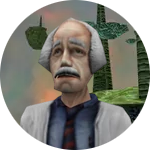
\includegraphics[width=3cm]{opening/resources/about/coomer.png} & \vspace{-0.5mm} {\large \thesisTutor} 
        \newline What a big fish you've got yourself. Show off your tutor. Now that's a job well done. Lorem ipsum dolor sit amet, consectetur adipiscing elit. Integer tempus quis elit id sagittis. Cras tincidunt nisi at tellus luctus, et congue dolor posuere. Aliquam suscipit felis sit amet lacus ultrices aliquet. Sed sagittis ultrices nisi, vel elementum elit dignissim non. Fusce faucibus ex at massa ultrices elementum.
        \vspace{2mm} 
        \newline
        \href{https://orcid.org/}{  % Link to your orcid
            \icon{\faOrcid}{10}{orcid-green}
        }
        \href{https://www.linkedin.com/}{  % Link to your linkedin
            \icon{\faLinkedinIn}{10}{linkedin-blue}
        }
        \href{https://github.com/}{  % Link to your github
            \icon{\faGithub}{10}{github-black}
        }
        \href{https://twitter.com/}{  % Link to your twitter
            \icon{\faTwitter}{10}{twitter-blue}
        }
        \href{mailto:example@domain.org}{  % Your E-mail
            \icon{\faEnvelope}{10}{email-red}
        }
        \href{https://t.me/}{  % Link to your telegram
            \icon{\faTelegramPlane}{10}{telegram-blue}
        }
    \end{tabular}
    
\endgroup





%%%%%%%%%%%%%%%%%%%%%%%%%%%%%%%%%%%%%%%%%%%%%%%%%%%%%%%%%%%%%%%%%%%%%%%%%%%%%%%%%%%%%%%%%%%%
% how to cite this work

% Listings workaround to include the background in broken lines

% \begin{verbatimwrite}{cite.txt}
% @mastersthesis{citeKey,
%     author  = "(*@{\thesisAuthor}@*) and (*@{\thesisTutor}@*)",
%     title   = "(*@{\thesisTitle}@*)",
%     school  = "(*@{\thesisSchool}@*)",
%     year    = "(*@{\thesisYear}@*)",
%     month   = "(*@{\thesisMonth}@*)",
%     address = "(*@{\thesisAddress}@*)"
% }
% \end{verbatimwrite}


\begingroup

\vspace*{\fill}

\small
\setlength\tabcolsep{0pt}
\renewcommand*{\arraystretch}{1.2}
{\noindent\large  Cite this work:}

% \begin{mdframed}[backgroundcolor=listing-background,hidealllines=true]
\vspace*{2mm}
% \lstinputlisting[style=cite, nolol]{./cite.txt}

\newwrite\tempfile
\immediate\openout\tempfile=cite.txt
\immediate\write\tempfile{%
@mastersthesis{citeKey,^^J
author  = "\thesisAuthor \space and \thesisTutor",^^J
title   = "\thesisTitle",^^J
school  = "\thesisSchool",^^J
year    = "\thesisYear",^^J
month   = "\thesisMonth",^^J
address = "\thesisAddress",^^J
type = "\thesisType"^^J
}
}
\immediate\closeout\tempfile

% Does not work because escapes are inside strings
% \begin{minted}{bibtex}
% @mastersthesis{citeKey,
%     author  = "¢{\thesisAuthor}¢ and ¢{\thesisTutor}¢",
%     title   = "¢{\thesisTitle}¢",
%     school  = "¢{\thesisSchool}¢",
%     year    = "¢{\thesisYear}¢",
%     month   = "¢{\thesisMonth}¢",
%     address = "¢{\thesisAddress}¢"
% }
% \end{minted}

\inputminted[style=algol_nu]{bibtex}{./cite.txt}
% \end{mdframed}


\endgroup


% Abstract
% 
%            ,,                                        
%          `7MM            _.o9                                
%            MM                                             
%  ,6"Yb.    MM  ,p6"bo   ,6"Yb.  M"""MMV  ,6"Yb.  `7Mb,od8 
% 8)   MM    MM 6M'  OO  8)   MM  '  AMV  8)   MM    MM' "' 
%  ,pm9MM    MM 8M        ,pm9MM    AMV    ,pm9MM    MM     
% 8M   MM    MM YM.    , 8M   MM   AMV  , 8M   MM    MM     
% `Moo9^Yo..JMML.YMbmd'  `Moo9^Yo.AMMmmmM `Moo9^Yo..JMML.   
% 
% 
% Free and Open-Source template for academic works
% https://github.com/dpmj/alcazar

\newpage

\clearpage
\cleardoublepage
\phantomsection

\pagestyle{plain}
\pagenumbering{gobble}

\phantomsection
\addcontentsline{toc}{chapter}{Abstract}

\begin{figure}
    \centering
    
\includegraphics[width=50px]{figures/logos/k8s-bw-2.png}
    \label{fig:abstract:kubernetes}
\end{figure}

\begin{center}
    \large \textbf{\thesisTitle}
\end{center}

{\noindent \textbf{\textsc{Keywords}}}

{\noindent \thesisKeywords}\\


{\noindent \textbf{\textsc{Abstract}}}

\noindent Il \glsname{ml} è una delle branche dell'informatica con le più complesse esigenze computazionali. La difficoltà intrinseca del realizzare modelli di machine learning si amplifica ulteriormente quando sorge la necessità - pressante e inevitabile - di traslare le fasi di sviluppo e di deployment ad un contesto distribuito. Grazie alla sua natura altamente parallelizzabile, i carichi di machine learning sono candidati ideale per i sistemi di orchestrazione di container, che fanno leva sulla scalabilità verticale per assicurare virtualmente un'infinita capacità computazionale.

Nell'ottica di questo lavoro di tesi, due modelli di machine learning dediti all'analisi genomica e realizzati con un paradigma monolitico sono stati sottoposti ad un processo di frammentazione in \glsname{microservizi} containerizzati. Avendo rilevato un sostanziale miglioramento delle performance del modello grazie alla sua nuova architettura, ci si è curati di trasportare la medesima su un cluster Kubernetes in grado di poterne gestire agilmente e con resilienza il ciclo di vita, dall'allenamento alla predizione, orchestrando queste fasi medianti Kubeflow. I risultati ottenuti trovano largo impiego sia su ecosistemi \textit{\glsname{cloudnative}} che \textit{\glsname{bm}}.

Al fine ultimo di tarare l'effettiva possibilità di trasferire in produzione quanto prodotto, è stata condotta un'analisi ad ampio spettro delle possibili vulnerabilità dell'architettura, immaginando molteplici scenari di attacco da parte di un avversario sulla rete. Quest'analisi ha permesso di valutare l'effettiva resilienza del sistema, e di proporre una serie di contromisure atte a mitigare i rischi individuati. Contestualmente, una serie di contributi sperimentali legati alla produzione di immagini Docker e alla loro distribuzione su un cluster Kubernetes sono stati proposti e discussi.

Lo studio condotto sottolinea il ruolo critico di Kubernetes nei sistemi ad alta complessità come quello presentato, ed evidenzia come il paradigma MLOps sia la modalità più organica e competitiva per sfruttare pienamente il potenziale del machine learning mediante l'adozione di architetture scalabili e resilienti con Kubernetes.

Uno spettro di possibili sviluppi futuri è stato osservato contestualmente all'attività progettuale: ad esempio, tecnologie come \glsname{mxnet}, \glsname{ray} o \glsname{mlflow} potrebbero costituire alternative valide a Kubeflow; inoltre, l'integrazione di strumenti di data governance come \glsname{fybrik} consentirebbe l'impiego di dataset contenenti PII, ampliando ulteriormente il campo di applicazione del sistema.

% Publications
%% 
%            ,,                                        
%          `7MM            _.o9                                
%            MM                                             
%  ,6"Yb.    MM  ,p6"bo   ,6"Yb.  M"""MMV  ,6"Yb.  `7Mb,od8 
% 8)   MM    MM 6M'  OO  8)   MM  '  AMV  8)   MM    MM' "' 
%  ,pm9MM    MM 8M        ,pm9MM    AMV    ,pm9MM    MM     
% 8M   MM    MM YM.    , 8M   MM   AMV  , 8M   MM    MM     
% `Moo9^Yo..JMML.YMbmd'  `Moo9^Yo.AMMmmmM `Moo9^Yo..JMML.   
% 
% 
% Free and Open-Source template for academic works
% https://github.com/dpmj/alcazar


% Add here your Publications.
% Depends on Biblatex and Biber for multiple bibliographies.

\newpage
\pagestyle{empty}

\clearpage
\cleardoublepage
\phantomsection

\pagestyle{empty}

% \phantomsection
% \addcontentsline{toc}{chapter}{Publications}


\begin{refsection}

    \nocite{own-article-1, own-article-2, own-article-3}

    \defbibnote{pre-note}{
        \noindent The {\thesisDegree} candidate, {\thesisAuthor}, has co-authored the following publications with Prof. {\thesisTutor} et al. The articles come as a result of the research activities carried out during the {\thesisType}. The candidate is the corresponding author in two of the three publications listed below:
    }
    \defbibnote{post-note}{
        \noindent Note: \cite{own-article-3} is not yet published.
    }

    \printbibliography[heading=bibintoc,  % Title in Table of contents
                       title={Publications},  % Title
                       prenote=pre-note,  % Text before bibliography
                       postnote=post-note]  % Text after bibliography

\end{refsection}


  % Optional: comment this line if you don't need it

% Acknowledgements
% 
%            ,,                                        
%          `7MM            _.o9                                
%            MM                                             
%  ,6"Yb.    MM  ,p6"bo   ,6"Yb.  M"""MMV  ,6"Yb.  `7Mb,od8 
% 8)   MM    MM 6M'  OO  8)   MM  '  AMV  8)   MM    MM' "' 
%  ,pm9MM    MM 8M        ,pm9MM    AMV    ,pm9MM    MM     
% 8M   MM    MM YM.    , 8M   MM   AMV  , 8M   MM    MM     
% `Moo9^Yo..JMML.YMbmd'  `Moo9^Yo.AMMmmmM `Moo9^Yo..JMML.   
% 
% 
% Free and Open-Source template for academic works
% https://github.com/dpmj/alcazar


% Add here your Acknowledgements. 
% This section is pretty free: free format, in one or various languages, etc.


\newpage
\thispagestyle{empty}

\clearpage
\cleardoublepage
\phantomsection

\pagestyle{plain}

\phantomsection
\addcontentsline{toc}{chapter}{Ringraziamenti}


\vspace*{\fill}

\begin{center}
    \large \textbf{\textsc{Ringraziamenti}}
\end{center}

Questa tesi di laurea magistrale corona il completamento di un percorso accademico quinquennale, disseminato da imprevisti, ostacoli, risultati dolceamari e traguardi che, un tempo, avrei ritenuto irraggiungibili. 

Nonostante l'esito di questo cammino umano e professionale, faccio ancora fatica a definirmi informatico. Durante gli ultimi due anni, ho avuto modo di interfacciarmi con individui di incredibile talento e immensa competenza. Grazie a loro, potrei aver finalmente capito cosa voglio fare nella vita.

Kevin Iuretig, Michele Di Giovanni e Francesco Foglia, con la loro straordinaria intelligenza e dedizione senza pari, hanno segnato il mio cammino professionale in maniera unica e personale. La loro acutissima curiosità e strepitosa intraprendenza hanno acceso la mia passione per il nostro mestiere, guidandomi attraverso sfide e successi. Molto dell'informatico che sono oggi lo devo a loro: per me, è un privilegio potermi considerare loro pari.

Questo percorso non sarebbe stato concretamente e fattualmente realizzabile senza un gruppo coeso e solido, mai sconfitto dal carico di studio né incrinato dal peso degli anni. Mentirei se affermassi che senza Dario Trinchese e Carmine Napolitano, preziosi colleghi e amici, sarei qui oggi a ponderare sul mio percorso post-universitario, poiché probabilmente sarebbe ancora molto distante. Inoltre, è indubbiamente grazie a loro se ho deciso in primo luogo di affrontare il percorso di laurea magistrale; a rendere, sento che non avrei potuto prendere una decisione migliore.

Infine, la mia famiglia, che mi ha sempre sostenuto e incoraggiato, non può che essere considerata la vera protagonista di questo percorso. Senza di loro, non sarei qui oggi a scrivere queste parole. Grazie.

\vspace*{\fill}



% Dedication
% To whom do you dedicate the thesis? Or maybe include a quote, poem, etc. Free space for yourself.
% Delete if you are too manly for these things
% 
%            ,,                                        
%          `7MM            _.o9                                
%            MM                                             
%  ,6"Yb.    MM  ,p6"bo   ,6"Yb.  M"""MMV  ,6"Yb.  `7Mb,od8 
% 8)   MM    MM 6M'  OO  8)   MM  '  AMV  8)   MM    MM' "' 
%  ,pm9MM    MM 8M        ,pm9MM    AMV    ,pm9MM    MM     
% 8M   MM    MM YM.    , 8M   MM   AMV  , 8M   MM    MM     
% `Moo9^Yo..JMML.YMbmd'  `Moo9^Yo.AMMmmmM `Moo9^Yo..JMML.   
% 
% 
% Free and Open-Source template for academic works
% https://github.com/dpmj/alcazar

\newpage
\thispagestyle{empty}

\clearpage
\cleardoublepage
\phantomsection

\thispagestyle{empty}

\phantomsection
\addcontentsline{toc}{chapter}{Dedication}



\vspace*{\fill}

\begin{flushright}

\textit{\large
\noindent A mia madre}
\end{flushright}



\vspace*{\fill}



% ------------------------------------------------------------------------------
% TABLES OF CONTENTS

\newpage
\thispagestyle{empty}

\clearpage
\cleardoublepage
\phantomsection

\pagestyle{plain}


\begingroup

    % Greatly compress space used by TOC, LOF and LOT
    \renewcommand{\baselinestretch}{1}  % less spacing
    \renewcommand{\contentsname}{Indice dei contenuti}
    \small  % smaller font size
    \setlength{\parskip}{0mm}  % Paragraph skip 0mm

    \pagenumbering{arabic}

    % List of Contents
    {
        \tableofcontents
        
        \addcontentsline{toc}{chapter}{Indice dei contenuti}
    }
    
    % List of Figures
    {
        \listoffigures
        \addcontentsline{toc}{chapter}{Indice delle figure}
    }
    
    % List of Tables
    {
        \listoftables
        \addcontentsline{toc}{chapter}{Indice delle tabelle}
    }
    
    % List of Listings -- uncomment if necessary
    {
        % \listoflistings
        % \addcontentsline{toc}{chapter}{List of listings}

        % \listof{lstlisting}{Code listings} % old code
    }
    
\endgroup

% END OPENING
% ------------------------------------------------------------------------------




% Chapters - main text
% 
%            ,,                                        
%          `7MM            _.o9                                
%            MM                                             
%  ,6"Yb.    MM  ,p6"bo   ,6"Yb.  M"""MMV  ,6"Yb.  `7Mb,od8 
% 8)   MM    MM 6M'  OO  8)   MM  '  AMV  8)   MM    MM' "' 
%  ,pm9MM    MM 8M        ,pm9MM    AMV    ,pm9MM    MM     
% 8M   MM    MM YM.    , 8M   MM   AMV  , 8M   MM    MM     
% `Moo9^Yo..JMML.YMbmd'  `Moo9^Yo.AMMmmmM `Moo9^Yo..JMML.   
% 
% 
% Free and Open-Source template for academic works
% https://github.com/dpmj/alcazar


% Start standard numbering and page style

\clearpage
\cleardoublepage
\phantomsection
\renewcommand\chaptername{Capitolo}

\pagestyle{chapters}
\setcounter{page}{1}

% 
%            ,,                                        
%          `7MM            _.o9                                
%            MM                                             
%  ,6"Yb.    MM  ,p6"bo   ,6"Yb.  M"""MMV  ,6"Yb.  `7Mb,od8 
% 8)   MM    MM 6M'  OO  8)   MM  '  AMV  8)   MM    MM' "' 
%  ,pm9MM    MM 8M        ,pm9MM    AMV    ,pm9MM    MM     
% 8M   MM    MM YM.    , 8M   MM   AMV  , 8M   MM    MM     
% `Moo9^Yo..JMML.YMbmd'  `Moo9^Yo.AMMmmmM `Moo9^Yo..JMML.   
% 
% 
% Free and Open-Source template for academic works
% https://github.com/dpmj/alca



\clearpage
\cleardoublepage

\chapter{Introduzione}

Questa tesi di laurea ha l'obiettivo di evidenziare le potenzialità di Kubernetes e dell'approccio distribuito ai problemi di Machine Learning, definendo una struttura concreta e organica per implementare pipeline completamente gestite ({\em "fully-managed"}) relative all'intero ciclo di vita dei modelli di machine learning. Verrà proposta un'analisi compilativa dello stato dell'arte strettamente correlato a questo contesto tecnologico, proponendo un contributo sperimentale legato alla trasformazione in microservizi di modelli monolitici pre-esistenti; successivamente, si esibirà un'analisi ad ampio spettro delle possibili vulnerabilità dell'architettura realizzata, fornendo anche in questo caso un contributo originale circa l'implementazione containerizzata di strumenti di attacco e ambienti vulnerabili.

Nel secondo capitolo, si presenterà un problema bioinformatico ad alta complessità relativo all'analisi genomica e alla classificazione dei geni di fusione, per i quali sono stati realizzati - nel contesto di altre tesi magistrali - due modelli di machine learning declinati in architetture monolitiche. Si descriveranno dunque le caratteristiche e il funzionamento a basso ed alto livello dei due modelli, evidenziando i difetti della loro attuale architettura.

Nel terzo capitolo, si delineeranno con formalità e precisione le tecnologie e gli strumenti informatici impiegati nei contesti distribuiti di Machine Learning. Si definiranno le principali convenzioni coinvolte, come le architetture a microservizi, e i concetti di orchestrazione, containerizzazione e virtualizzazione. Si descriveranno strumenti specifici finalizzati all'orchestrazione di generici carichi di lavoro, come \glsname{kubernetes}, proponendo poi anche uno strumento specifico ai carichi di Machine Learning, quale \glsname{kubeflow}. Si analizzeranno le architetture a basso livello di ambo le tecnologie per comprenderne a pieno le funzionalità, discutendo inoltre di come poter iterare sulle medesime attraverso lo sviluppo di componenti e pipeline di Machine Learning ex novo. Si accennerà brevemente a possibili alternative a Kubeflow, come \glsname{mxnet}, \glsname{ray} e \glsname{mlflow}, nonché ad alcuni possibili provider di cloud computing (\glsname{aws}, \glsname{gcp}) che offrono servizi completamente gestiti per i cluster Kubernetes.

Nel quarto capitolo, i modelli descritti nel secondo capitolo subiranno una trasformazione in microservizi così come proposto nel terzo capitolo, sfruttando Kubernetes e Kubeflow per lo sviluppo delle pipeline distribuite. L'intero processo, opportunamento documentato, esibirà le sue potenzialità in un benchmark delle prestazioni, rilevando un miglioramento notevole dei tempi di esecuzione. Inoltre, si delineeranno le modalità di integrazione di driver CUDA per l'utilizzo della GPU nelle fasi di training e testing, e il funzionamento di registry di immagini Docker on-premise.

Nel quinto capitolo, si avanzeranno una serie di considerazioni compilative e sperimentali di \glsname{mlsecops}. In particolare, veranno impiegate tecnologie allo stato dell'arte, come \glsname{metasploit}, \glsname{kali}, \glsname{cdk} e \glsname{artillery}, per tarare e penetrare le difese dell'infrastruttura realizzata, esponendone vulnerabilità per poi mitigare i rischi di intrusione. Sono inoltre proposti ulteriori contributi sperimentali, contestuali a questo lavoro di tesi, circa la produzione di immagini Docker degli strumenti indicati. 

Nel sesto capitolo, vengono delineati i possibili sviluppi futuri che potrebbero permette di traslare in produzione l'infrastruttura presentata. In particolare, si accenna alla possibilità di integrare tecniche di \glsname{mlre} e \glsname{datagovernance} per amplificare la sicurezza e resilienza del sistema; inoltre, si individua in \glsname{helm} una possibile modalità di distribuzione dell'architettura come applicazione Kubernetes portabile.

\section{La Rivoluzione DevOps e le sue conseguenze}

Il Movimento \glsname{devops}, nato dalla convergenza tra "development" e "operations", si è delineato come risposta alle sfide emergenti nel ciclo di vita dello sviluppo del software. Il suo percorso evolutivo può essere tracciato attraverso una serie di fasi che hanno modellato e influenzato la sua crescita.

\begin{figure}[h]
    \centering
    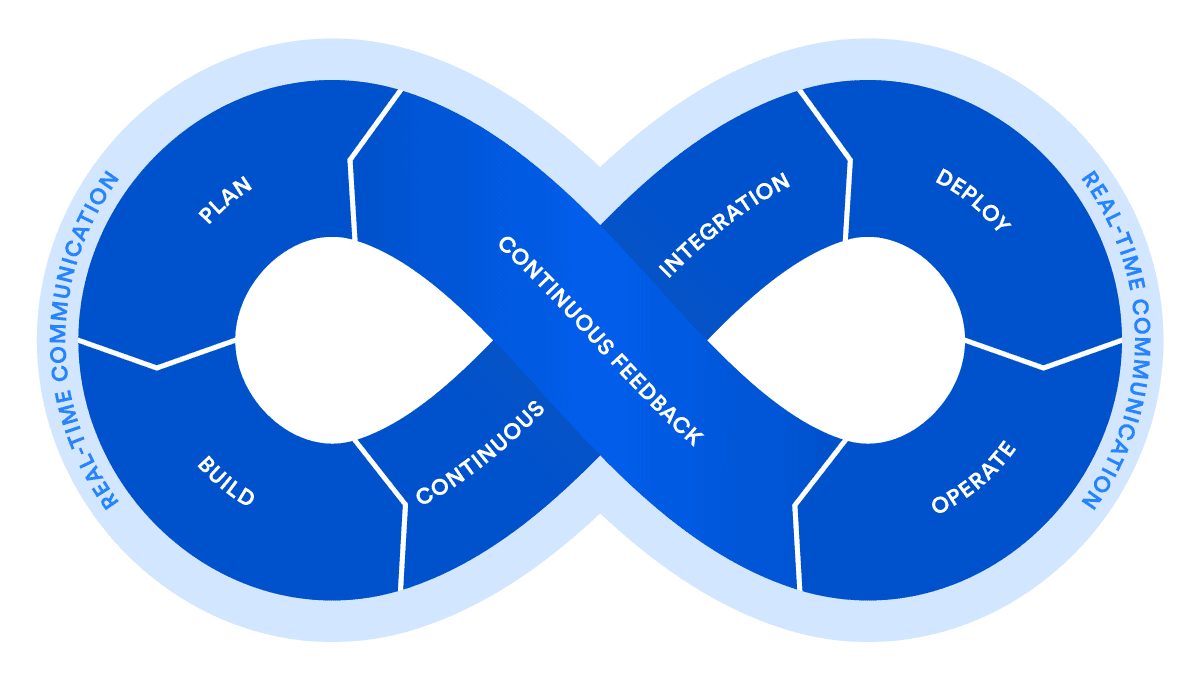
\includegraphics[width=200px]{figures/ch1/devops-flow.png}
    \caption[Development \& Operations: un'icona del movimento DevOps]{Development \& Operations: un'icona del movimento DevOps}
    \label{fig:cha1:devops}
\end{figure}

Negli anni 2000, le crescenti complessità delle applicazioni e la necessità di cicli di rilascio più rapidi hanno reso evidente la necessità di una collaborazione più stretta tra team di sviluppo e team operativo, inteso come l'insieme di tecnici e ingegneri dediti alla distribuzione delle applicazioni e al mantenimento delle pipeline di rilascio. Questo periodo ha visto la formazione di una consapevolezza crescente dell'importanza di superare le barriere tradizionali tra queste due squadre distinte.

\begin{figure}[h]
    \centering
    \subfloat["The Phoenix Project" (2013)]["The Phoenix Project" (2013)]{
        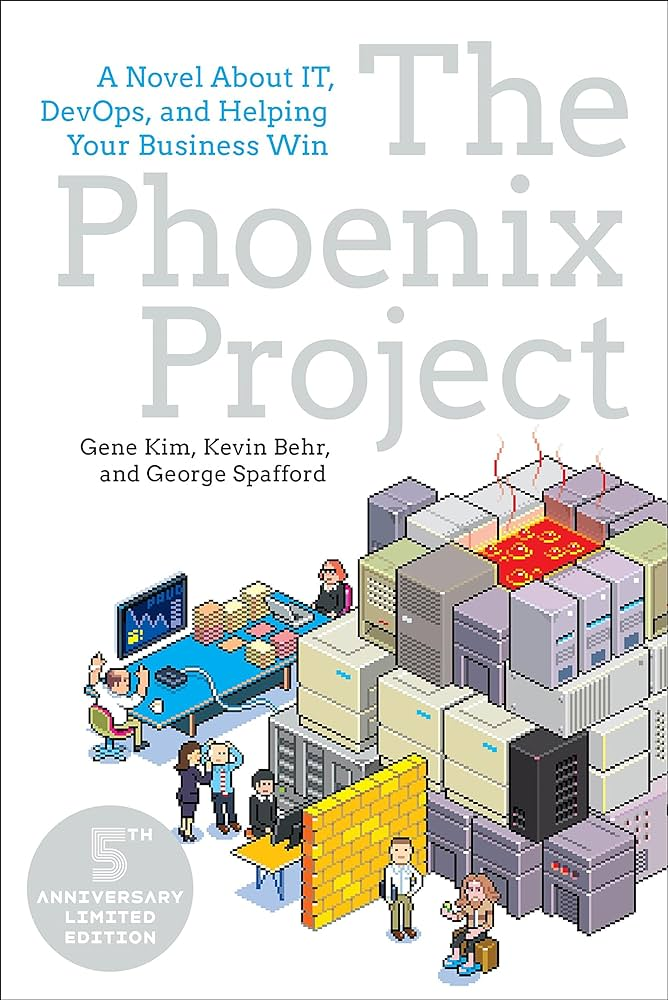
\includegraphics[width=150px]{figures/ch1/phoenix_project.jpg}
            \label{fig:cha1:unicorn}
    }
    \hspace{30px}
    \subfloat["The Unicorn Project" (2019)]["The Unicorn Project" (2019)]{
        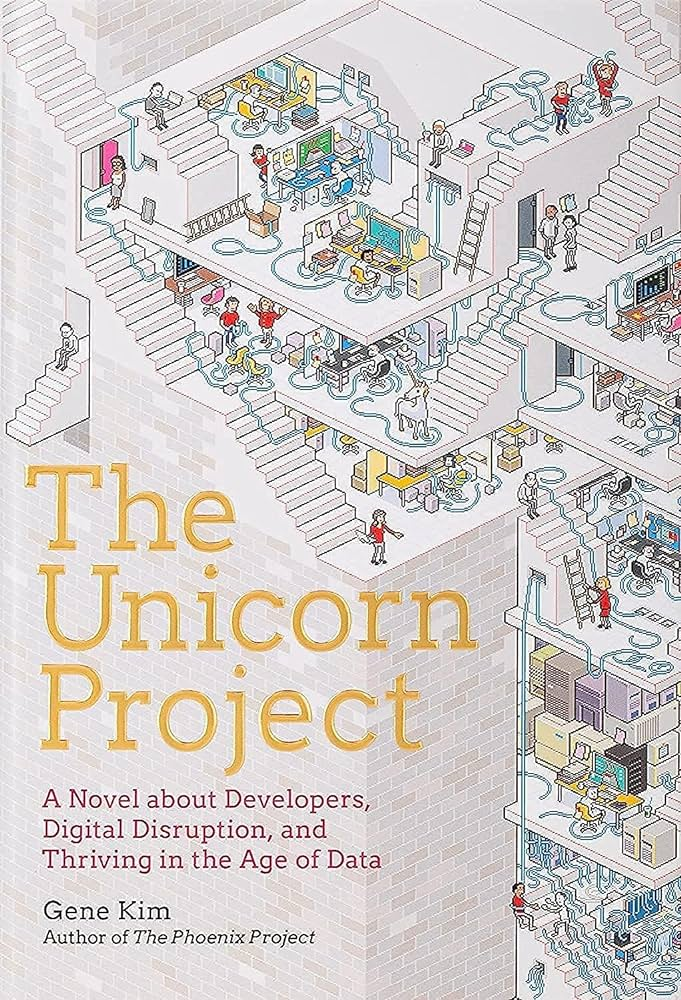
\includegraphics[width=150px]{figures/ch1/unicorn_project.jpg}
            \label{fig:cha1:phoenix}
    }
    \caption{Copertine di "The Phoenix Project" e "The Unicorn Project"}
    \label{fig:cha1:jerez}
\end{figure}

Il termine "{\em DevOps}" è stato coniato nel 2009 durante una conferenza a Bruxelles, segnando un punto di svolta nel modo in cui le organizzazioni affrontano le sfide della distribuzione software. Patrick Debois e Andrew Shafer sono stati tra i pionieri di questa iniziativa, cercando di superare i conflitti tra sviluppatori e operatori.

Negli anni successivi, il Movimento DevOps ha iniziato a focalizzarsi sulla definizione di pratiche e principi chiave, con l'obiettivo di migliorare la collaborazione, la trasparenza e la velocità di rilascio. Il libro "The Phoenix Project" \cite{phoenix} di Gene Kim, Kevin Behr e George Spafford (2013) ha contribuito a diffondere i concetti fondamentali del movimento DevOps, enfatizzando la cultura ingegneristica, l'automazione, la misurazione delle performance e il miglioramento continuo delle competenze (CALMS).

La diffusione del movimento DevOps è stata accompagnata dall'adozione di strumenti e pratiche di automazione. Strumenti come Puppet, Chef e Ansible hanno semplificato la gestione delle configurazioni, mentre Jenkins ha rivoluzionato la pratica dell'integrazione continua.

Negli ultimi anni, il movimento DevOps è diventato uno standard industriale \cite{devops_1}, adottato da un numero sempre maggiore di organizzazioni. L'integrazione di pratiche DevOps è diventata un requisito chiave per affrontare l'accelerazione della domanda di rilasci software e la necessità di rispondere rapidamente ai cambiamenti del mercato.

L'adozione di pratiche DevOps ha portato a benefici tangibili \cite{devops_2}, come la riduzione dei tempi di rilascio, il miglioramento della qualità del software e un maggiore allineamento tra sviluppo e operazioni. Tuttavia, la complessità nell'implementare con successo DevOps in ambienti eterogenei e la gestione del cambiamento culturale rimangono sfide significative.

\begin{figure}[h]
    \centering
    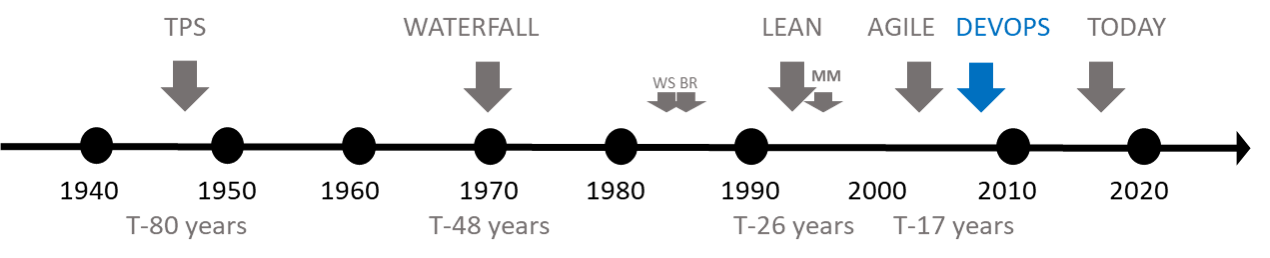
\includegraphics[width=400px]{figures/ch1/devops-timeline.png}
    \caption[Timeline dei metodi di sviluppo nell'industria IT]{Timeline dei metodi di sviluppo nell'industria IT}
    \label{fig:cha1:from_waterfall_to_devops}
\end{figure}

Il Movimento DevOps rappresenta un'evoluzione fondamentale nel modo in cui le organizzazioni affrontano lo sviluppo e il rilascio del software. Dalla sua nascita agli sviluppi recenti, DevOps ha continuato a plasmare il panorama tecnologico e culturale delle aziende, dimostrando la sua essenzialità nell'era della trasformazione digitale.

\section{I paradigmi MLOps e MLSecOps}

Il paradigma \glsname{mlops} ({\em Machine Learning Operations}) e il paradigma \glsname{mlsecops} ({\em Machine Learning Security Operations}) costituiscono una sinergia evolutiva nell'ambito della gestione delle operazioni e della sicurezza nell'implementazione di soluzioni basate su machine learning. Il loro sviluppo è radicato in una cornice storica che riflette l'espansione crescente e la complessità delle applicazioni di intelligenza artificiale (IA) e di machine learning (ML).

\begin{figure}[h]
    \centering
    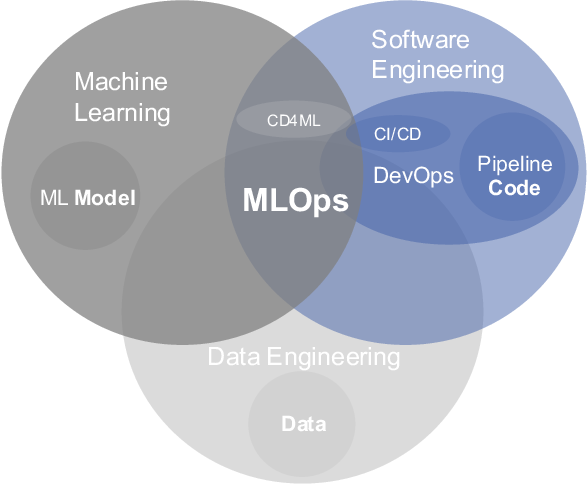
\includegraphics[width=200px]{figures/ch1/mlops-flow.png}
    \caption[Intersezione fra Machine Learning, DevOps e Data Engineering]{Collocamento della branca MLOps nell'informatica}
    \label{fig:cha1:mlops}
\end{figure}

Il paradigma MLOps \cite{mlops} trova le sue radici nella necessità di affrontare le sfide operative emergenti nella gestione di modelli di machine learning su larga scala. Nel corso degli anni, l'adozione di modelli ML è cresciuta esponenzialmente, portando alla comparsa di problemi legati alla distribuzione, all'aggiornamento e al monitoraggio dei modelli in produzione. Il concetto di MLOps ha preso forma attraverso l'esperienza pratica e la risposta alle esigenze operative emergenti nell'industria.

Similmente, il paradigma MLSecOps ha avuto origine dall'urgente necessità di mitigare i rischi legati alla sicurezza nell'ambito dei modelli di machine learning \cite{adv_ml_1}. La crescente consapevolezza delle vulnerabilità specifiche dei modelli ML, come gli attacchi di avversarial machine learning, ha stimolato la nascita di MLSecOps. Questo paradigma mira a integrare le pratiche di sicurezza nell'intero ciclo di vita dei modelli, dalla fase di sviluppo alla fase operativa.

Le motivazioni sottese al paradigma MLOps si concentrano sulla necessità di automatizzare e semplificare il ciclo di vita dei modelli ML, garantendo un deployment efficiente, la gestione delle versioni, il monitoraggio continuo e l'aggiornamento senza intoppi dei modelli in produzione. Il paradigma MLOps si propone di risolvere le sfide operative, garantendo la coerenza tra gli ambienti di sviluppo e produzione, nonché la riproducibilità e la tracciabilità dei risultati.

Dall'altro lato, il paradigma MLSecOps è guidato dalla volontà di proteggere i modelli di machine learning da minacce e attacchi. Ciò implica l'implementazione di misure di sicurezza proattive durante lo sviluppo, nonché la continua valutazione della robustezza dei modelli in produzione. La necessità di comprendere e mitigare le vulnerabilità specifiche dei modelli ML, che possono essere sfruttate da attaccanti astuti, è al centro del paradigma MLSecOps.

I vantaggi del paradigma MLOps sono molteplici e si riflettono nella migliorata efficienza operativa, nella riduzione dei tempi di deployment e nella gestione semplificata delle versioni dei modelli. L'implementazione di pratiche MLOps consente una transizione fluida dai prototipi agli ambienti di produzione, garantendo un flusso di lavoro ottimizzato e una risposta rapida alle esigenze del business.

L'evoluzione del paradigma il paradigma MLOps è strettamente connessa all'avanzamento delle tecnologie che ne supportano l'implementazione. L'adozione di strumenti di automazione, gestione del ciclo di vita e orchestrazione dei modelli ha ridefinito il panorama delle operazioni di machine learning. In particolare, piattaforme come Ray \cite{ray}, MLflow \cite{mlflow} e Kubeflow \cite{kubeflow} hanno svolto un ruolo cruciale nella standardizzazione e semplificazione del flusso di lavoro MLOps.

Tuttavia, è cruciale riconoscere che l'adozione del paradigma MLOps non è esente da sfide. La complessità nell'orchestrare processi di machine learning su vasta scala, la gestione delle dipendenze e la necessità di un monitoraggio continuo possono presentare ostacoli significativi.

Per quanto riguarda il paradigma MLSecOps, i suoi vantaggi sono evidenti nella capacità di proteggere i modelli ML da minacce e attacchi, preservando l'integrità e la riservatezza dei dati. L'integrazione di pratiche di sicurezza fin dalla fase di sviluppo contribuisce a ridurre il rischio di vulnerabilità e garantisce una maggiore fiducia nella robustezza dei modelli.

Tuttavia, anche il paradigma MLSecOps non è immune da sfide \cite{adv_ml_2}. La continua evoluzione delle tecniche di attacco richiede un costante adattamento delle misure di sicurezza, e la complessità degli algoritmi di machine learning può rendere difficile la previsione e la mitigazione di potenziali minacce.

I paradigmi MLOps e MLSecOps rappresentano risposte essenziali alle sfide emergenti nella implementazione di soluzioni di machine learning su larga scala. Mentre l'idea attorno al paradigma MLOps si concentra sull'ottimizzazione delle operazioni di distribuzione di applicativi di machine learning, il paradigma MLSecOps mira a garantire la sicurezza dei modelli di machine learning. L'implementazione sinergica di entrambi i paradigmi può contribuire a un ecosistema ML resiliente e efficiente.

%% 
%            ,,                                        
%          `7MM            _.o9                                
%            MM                                             
%  ,6"Yb.    MM  ,p6"bo   ,6"Yb.  M"""MMV  ,6"Yb.  `7Mb,od8 
% 8)   MM    MM 6M'  OO  8)   MM  '  AMV  8)   MM    MM' "' 
%  ,pm9MM    MM 8M        ,pm9MM    AMV    ,pm9MM    MM     
% 8M   MM    MM YM.    , 8M   MM   AMV  , 8M   MM    MM     
% `Moo9^Yo..JMML.YMbmd'  `Moo9^Yo.AMMmmmM `Moo9^Yo..JMML.   
% 
% 
% Free and Open-Source template for academic works
% https://github.com/dpmj/alcazar



\clearpage
\cleardoublepage

\chapter{Specifications}

\section{Aljibe}

This is an example of how this template may be used. As we can see in \autoref{fig:cha1:donpedro}, the \glsname{jupyter} is lorem ipsum dolor sit amet  \cite{ESP32_DATASHEET}, consectetur adipiscing elit. Integer tempus quis elit id sagittis. Cras tincidunt nisi at tellus luctus, et congue dolor posuere. Aliquam suscipit felis sit amet lacus ultrices aliquet. 

Sed sagittis ultrices nisi, vel elementum elit dignissim non. Fusce faucibus ex at massa ultrices elementum. Nullam ullamcorper lorem sit amet facilisis cursus. Suspendisse non erat non justo porta placerat. Morbi porttitor dictum molestie. \glsname{adiabatic} sed vitae iaculis libero. Suspendisse in gravida lacus, tempor ultrices nibh. Nam consequat scelerisque porttitor \cite{SOLDERDEFECTS}.

\subsection{Alberca}

\subsubsection{Nullam quis lacus}

Nullam quis lacus vel ante feugiat efficitur id ut quam. Pellentesque commodo elit nec urna gravida maximus. Suspendisse ut risus eu ipsum porta porta ac et orci. Donec dictum ligula sodales, euismod est sed, semper libero. In blandit, nulla et elementum pharetra, mi nunc sagittis tellus, sit amet scelerisque magna elit ac sapien. Curabitur ipsum dui, pretium a maximus id, varius gravida nisl. Sed vitae mattis elit, vitae hendrerit lorem

Lorem ipsum dolor sit amet, consectetur adipiscing elit. Integer tempus quis elit id sagittis. Cras tincidunt nisi at tellus luctus, et congue dolor posuere. Aliquam suscipit felis sit amet lacus ultrices aliquet . Sed sagittis ultrices nisi, vel elementum elit dignissim non. Fusce faucibus ex at massa ultrices elementum. Nullam ullamcorper lorem sit amet facilisis cursus. Suspendisse non erat non justo porta placerat. Morbi porttitor dictum molestie. Sed vitae iaculis libero. Suspendisse in gravida lacus, tempor ultrices nibh. Nam consequat scelerisque porttitor.

\subsubsection{Nulla elementum orci}

Nulla elementum orci in dolor dapibus, ac facilisis sem ultrices. Nullam eleifend id eros sed luctus. Maecenas arcu ipsum, scelerisque id lorem in, placerat posuere tellus. Etiam gravida velit sed arcu viverra dapibus. Mauris vitae augue dapibus, molestie justo eget, condimentum ipsum. Nulla tristique mi eget semper luctus. Etiam commodo vestibulum vulputate. Etiam quis sapien dolor. Nunc tristique eu lacus quis ullamcorper. Sed volutpat rutrum vehicula. Donec nunc nisl, suscipit in faucibus vitae, tristique eu risus. Nulla facilisis augue eget


\begin{table}
    \small
    \centering
    \renewcommand{\arraystretch}{1.5}
    \begin{tabular}{|cccccc|}
    \hline
    \rowcolor{lightgray}\multicolumn{6}{|c|}{\textbf{Voltage of internal LDO (VDD\_SDIO)}} \\ \hline
    \multicolumn{1}{|c|}{Pin} & \multicolumn{1}{c|}{Default} & \multicolumn{2}{c|}{VDD\_SDIO = 3.3 V} & \multicolumn{2}{c|}{VDD\_SDIO = 1.8 V} \\ \hline
    \multicolumn{1}{|c|}{GPIO12/MTDI} & \multicolumn{1}{c|}{Pull-down} & \multicolumn{2}{c|}{0} & \multicolumn{2}{c|}{1} \\ \hline\hline
    
    \rowcolor{lightgray}\multicolumn{6}{|c|}{\textbf{Booting mode}} \\ \hline
    \multicolumn{1}{|c|}{Pin} & \multicolumn{1}{c|}{Default} & \multicolumn{2}{c|}{SPI boot} & \multicolumn{2}{c|}{Download boot (programming)} \\ \hline
    \multicolumn{1}{|c|}{GPIO0} & \multicolumn{1}{c|}{Pull-up} & \multicolumn{2}{c|}{1} & \multicolumn{2}{c|}{0} \\ \hline
    \multicolumn{1}{|c|}{GPIO2} & \multicolumn{1}{c|}{Pull-down} & \multicolumn{2}{c|}{Don't care} & \multicolumn{2}{c|}{0} \\ \hline\hline
    
    \rowcolor{lightgray}\multicolumn{6}{|c|}{\textbf{Enabling/Disabling debugging log print over UOTXD (UART TXD) during boot}} \\ \hline
    \multicolumn{1}{|c|}{Pin} & \multicolumn{1}{c|}{Default} & \multicolumn{2}{c|}{U0TXD Active} & \multicolumn{2}{c|}{U0TXD Silent} \\ \hline
    \multicolumn{1}{|c|}{GPIO15/MTDO} & \multicolumn{1}{c|}{Pull-up} & \multicolumn{2}{c|}{1} & \multicolumn{2}{c|}{0} \\ \hline\hline
    
    \rowcolor{lightgray}\multicolumn{6}{|c|}{\textbf{Timing of SDIO slave}} \\ \hline
    \multicolumn{1}{|c|}{Pin} & \multicolumn{1}{c|}{Default} & \multicolumn{1}{c|}{\begin{tabular}[c]{@{}c@{}}FE Sampling\\FE Output\end{tabular}} & \multicolumn{1}{c|}{\begin{tabular}[c]{@{}c@{}}FE Sampling\\RE Output\end{tabular}} & \multicolumn{1}{c|}{\begin{tabular}[c]{@{}c@{}}RE Sampling\\FE Output\end{tabular}} & \begin{tabular}[c]{@{}c@{}}RE Sampling\\RE Output\end{tabular} \\ \hline
    \multicolumn{1}{|c|}{GPIO15/MTDO} & \multicolumn{1}{c|}{Pull-up} & \multicolumn{1}{c|}{0} & \multicolumn{1}{c|}{0} & \multicolumn{1}{c|}{1} & 1 \\ \hline
    \multicolumn{1}{|c|}{GPIO5} & \multicolumn{1}{c|}{Pull-up} & \multicolumn{1}{c|}{0} & \multicolumn{1}{c|}{1} & \multicolumn{1}{c|}{0} & 1 \\ \hline
    \end{tabular}
    \caption[Strapping pin configuration during boot on the ESP32.]{Strapping pin configuration during boot on the ESP32. Extracted from ESP32's data sheet \cite{ESP32_DATASHEET} (Table 5, page 21). FE: Falling Edge, RE: Rising Edge.}
    \label{tab:design:circuit:esp32:strapping_pins}
    \end{table}


\subsubsection{Nullam quis lacus}

Nullam quis lacus vel ante feugiat efficitur id ut quam. Pellentesque commodo elit nec urna gravida maximus. Suspendisse ut risus eu ipsum porta porta ac et orci. Donec dictum ligula sodales, euismod est sed, semper libero. In blandit, nulla et elementum pharetra, mi nunc sagittis tellus, sit amet scelerisque magna elit ac sapien. Curabitur ipsum dui, pretium a maximus id, varius gravida nisl. Sed vitae mattis elit, vitae hendrerit lorem.

Lorem ipsum dolor sit amet, consectetur adipiscing elit. Integer tempus quis elit id sagittis. Cras tincidunt nisi at tellus luctus, et congue dolor posuere. Aliquam suscipit felis sit amet lacus ultrices aliquet. Sed sagittis ultrices nisi, vel elementum elit dignissim non. Fusce faucibus ex at massa ultrices elementum. Nullam ullamcorper lorem sit amet facilisis cursus. Suspendisse non erat non justo porta placerat. Morbi porttitor dictum molestie. Sed vitae iaculis libero. Suspendisse in gravida lacus, tempor ultrices nibh. Nam consequat scelerisque porttitor.

\subsubsection{Nulla elementum orci}

Nulla elementum orci in dolor dapibus, ac facilisis sem ultrices. Nullam eleifend id eros sed luctus. Maecenas arcu ipsum, scelerisque id lorem in, placerat posuere tellus. Etiam gravida velit sed arcu viverra dapibus. Mauris vitae augue dapibus, molestie justo eget, condimentum ipsum. Nulla tristique mi eget semper luctus. Etiam commodo vestibulum vulputate. Etiam quis sapien dolor. Nunc tristique eu lacus quis ullamcorper. Sed volutpat rutrum vehicula. Donec nunc nisl, suscipit in faucibus vitae, tristique eu risus. Nulla facilisis augue eget


\section{Acequia}

\subsection{Nulla elementum orci}

Nulla elementum orci in dolor dapibus, ac facilisis sem ultrices. Nullam eleifend id eros sed luctus. Maecenas arcu ipsum, scelerisque id lorem in, placerat posuere tellus. Etiam gravida velit sed arcu viverra dapibus. Mauris vitae augue dapibus, molestie justo eget, condimentum ipsum. Nulla tristique mi eget semper luctus. Etiam commodo vestibulum vulputate. Etiam quis sapien dolor. Nunc tristique eu lacus quis ullamcorper. Sed volutpat rutrum vehicula. Donec nunc nisl, suscipit in faucibus vitae, tristique eu risus. Nulla facilisis augue eget


\subsubsection{Nullam quis lacus}

Nullam quis lacus vel ante feugiat efficitur id ut quam. Pellentesque commodo elit nec urna gravida maximus. Suspendisse ut risus eu ipsum porta porta ac et orci. Donec dictum ligula sodales, euismod est sed, semper libero. In blandit, nulla et elementum pharetra, mi nunc sagittis tellus, sit amet scelerisque magna elit ac sapien. Curabitur ipsum dui, pretium a maximus id, varius gravida nisl. Sed vitae mattis elit, vitae hendrerit lorem.

Lorem ipsum dolor sit amet, consectetur adipiscing elit. Integer tempus quis elit id sagittis. Cras tincidunt nisi at tellus luctus, et congue dolor posuere. Aliquam suscipit felis sit amet lacus ultrices aliquet. Sed sagittis ultrices nisi, vel elementum elit dignissim non. Fusce faucibus ex at massa ultrices elementum. Nullam ullamcorper lorem sit amet facilisis cursus. Suspendisse non erat non justo porta placerat. Morbi porttitor dictum molestie. Sed vitae iaculis libero. Suspendisse in gravida lacus, tempor ultrices nibh. Nam consequat scelerisque porttitor.

\subsubsection{Nulla elementum orci}

Nulla elementum orci in dolor dapibus, ac facilisis sem ultrices. Nullam eleifend id eros sed luctus. Maecenas arcu ipsum, scelerisque id lorem in, placerat posuere tellus. Etiam gravida velit sed arcu viverra dapibus. Mauris vitae augue dapibus, molestie justo eget, condimentum ipsum. Nulla tristique mi eget semper luctus. Etiam commodo vestibulum vulputate. Etiam quis sapien dolor. Nunc tristique eu lacus quis ullamcorper. Sed volutpat rutrum vehicula. Donec nunc nisl, suscipit in faucibus vitae, tristique eu risus. Nulla facilisis augue eget


% Glossary and acronyms
% 
%            ,,                                        
%          `7MM            _.o9                                
%            MM                                             
%  ,6"Yb.    MM  ,p6"bo   ,6"Yb.  M"""MMV  ,6"Yb.  `7Mb,od8 
% 8)   MM    MM 6M'  OO  8)   MM  '  AMV  8)   MM    MM' "' 
%  ,pm9MM    MM 8M        ,pm9MM    AMV    ,pm9MM    MM     
% 8M   MM    MM YM.    , 8M   MM   AMV  , 8M   MM    MM     
% `Moo9^Yo..JMML.YMbmd'  `Moo9^Yo.AMMmmmM `Moo9^Yo..JMML.   
% 
% 
% Free and Open-Source template for academic works
% https://github.com/dpmj/alcazar


%%%%%%%%%%%%%%%%%%%%%%%%%%%%%%%%%%%%%%%%%%%%%%%%%%%%%%%%%%%%%%%%%%%%%%%%%%%%%%%%%%%%%%%%%%%
% GLOSSARY


\clearpage
\cleardoublepage
\phantomsection

\renewcommand*{\glossaryname}{Glossario}%

{
    \small
    \printglossaries
}


% Bibliography
% 
%            ,,                                        
%          `7MM            _.o9                                
%            MM                                             
%  ,6"Yb.    MM  ,p6"bo   ,6"Yb.  M"""MMV  ,6"Yb.  `7Mb,od8 
% 8)   MM    MM 6M'  OO  8)   MM  '  AMV  8)   MM    MM' "' 
%  ,pm9MM    MM 8M        ,pm9MM    AMV    ,pm9MM    MM     
% 8M   MM    MM YM.    , 8M   MM   AMV  , 8M   MM    MM     
% `Moo9^Yo..JMML.YMbmd'  `Moo9^Yo.AMMmmmM `Moo9^Yo..JMML.   
% 
% 
% Free and Open-Source template for academic works
% https://github.com/dpmj/alcazar


\clearpage
\cleardoublepage

\pagestyle{biblio}


\renewcommand\bibname{Bibliografia}
\phantomsection
\addcontentsline{toc}{chapter}{Bibliografia}

{
    \renewcommand{\UrlFont}{\ttfamily\scriptsize}  
    % Smaller URLs (USE FOR IBM PLEX MONO ONLY)

    \small  % Compress space used by bibliography

    % For bibtex bibliography
    % \bibliographystyle{ieeetr}
    % \bibliography{bibliography/eferences

    % Multi-column bibliography 
    % For biblatex bibliography
    \begin{multicols}{2}[\printbibheading]
        \AtNextBibliography{\small \pagestyle{biblio}}
        \printbibliography[heading=none]
    \end{multicols}

}


% Addendum - secondary text
%% 
%            ,,                                        
%          `7MM            _.o9                                
%            MM                                             
%  ,6"Yb.    MM  ,p6"bo   ,6"Yb.  M"""MMV  ,6"Yb.  `7Mb,od8 
% 8)   MM    MM 6M'  OO  8)   MM  '  AMV  8)   MM    MM' "' 
%  ,pm9MM    MM 8M        ,pm9MM    AMV    ,pm9MM    MM     
% 8M   MM    MM YM.    , 8M   MM   AMV  , 8M   MM    MM     
% `Moo9^Yo..JMML.YMbmd'  `Moo9^Yo.AMMmmmM `Moo9^Yo..JMML.   
% 
% 
% Free and Open-Source template for academic works
% https://github.com/dpmj/alcazar



\clearpage
\cleardoublepage


\begin{appendices}

    \pagestyle{addenda}

    \renewcommand\chaptername{Appendix}  
    % Change name of the chapters
    % This is necessary due to a conflict with titlesec package


    % 
%            ,,                                        
%          `7MM            _.o9                                
%            MM                                             
%  ,6"Yb.    MM  ,p6"bo   ,6"Yb.  M"""MMV  ,6"Yb.  `7Mb,od8 
% 8)   MM    MM 6M'  OO  8)   MM  '  AMV  8)   MM    MM' "' 
%  ,pm9MM    MM 8M        ,pm9MM    AMV    ,pm9MM    MM     
% 8M   MM    MM YM.    , 8M   MM   AMV  , 8M   MM    MM     
% `Moo9^Yo..JMML.YMbmd'  `Moo9^Yo.AMMmmmM `Moo9^Yo..JMML.   
% 
% 
% Free and Open-Source template for academic works
% https://github.com/dpmj/alcazar


% Example of an appendix


\chapter{Something vaguely related to the main content, but you put a lot of effort into it.}


\section{Praesent vulputate tellus vel metus rutrum}


Lorem ipsum dolor sit amet, consectetur adipiscing elit. Integer tempus quis elit id sagittis. Cras tincidunt nisi at tellus luctus, et congue dolor posuere. Aliquam suscipit felis sit amet lacus ultrices aliquet. Sed sagittis ultrices nisi, vel elementum elit dignissim non. Fusce faucibus ex at massa ultrices elementum. Nullam ullamcorper lorem sit amet facilisis cursus. Suspendisse non erat non justo porta placerat. Morbi porttitor dictum molestie. Sed vitae iaculis libero. Suspendisse in gravida lacus, tempor ultrices nibh. Nam consequat scelerisque porttitor \cite{europa_rohs, europa_ce}.


\subsection{Faucibus interdum nisi}

Nulla elementum orci in dolor dapibus, ac facilisis sem ultrices. Nullam eleifend id eros sed luctus. Maecenas arcu ipsum, scelerisque id lorem in, placerat posuere tellus \cite{proceedings_piezo}. Etiam gravida velit sed arcu viverra dapibus. Mauris vitae augue dapibus, molestie justo eget, condimentum ipsum. Nulla tristique mi eget semper luctus. Etiam commodo vestibulum vulputate. Etiam quis sapien dolor. Nunc tristique eu lacus quis ullamcorper. Sed volutpat rutrum vehicula. Donec nunc nisl, suscipit in faucibus vitae, tristique eu risus. \glsname{GNU} nulla facilisis augue eget interdum rutrum. Aliquam sem nunc, fermentum sed urna ac, faucibus interdum nisi.


\subsection{Praesent vulputate tellus vel metus rutrum}

Proin a condimentum nibh. Praesent vulputate tellus vel metus rutrum, non luctus mi sollicitudin. Nam ac tellus ut eros sollicitudin luctus at ac mi. Vestibulum mollis nec nisi a laoreet. Proin neque tortor, placerat nec suscipit sit amet, ullamcorper in sem. Fusce faucibus ultrices cursus. Maecenas scelerisque mauris diam, at volutpat nisi porta vitae. 

Sed at ipsum et leo cursus varius eu eu lectus. Class aptent taciti sociosqu ad litora torquent per conubia nostra, per inceptos himenaeos. 

Ut felis ipsum, imperdiet rhoncus orci ac, consectetur luctus nisl. Cras aliquet elementum tellus ullamcorper malesuada. Integer purus est, pharetra eu ullamcorper quis, imperdiet non turpis. \cite{SOFTWARE_ENGINEERING_9}




\begin{figure}
    \centering
    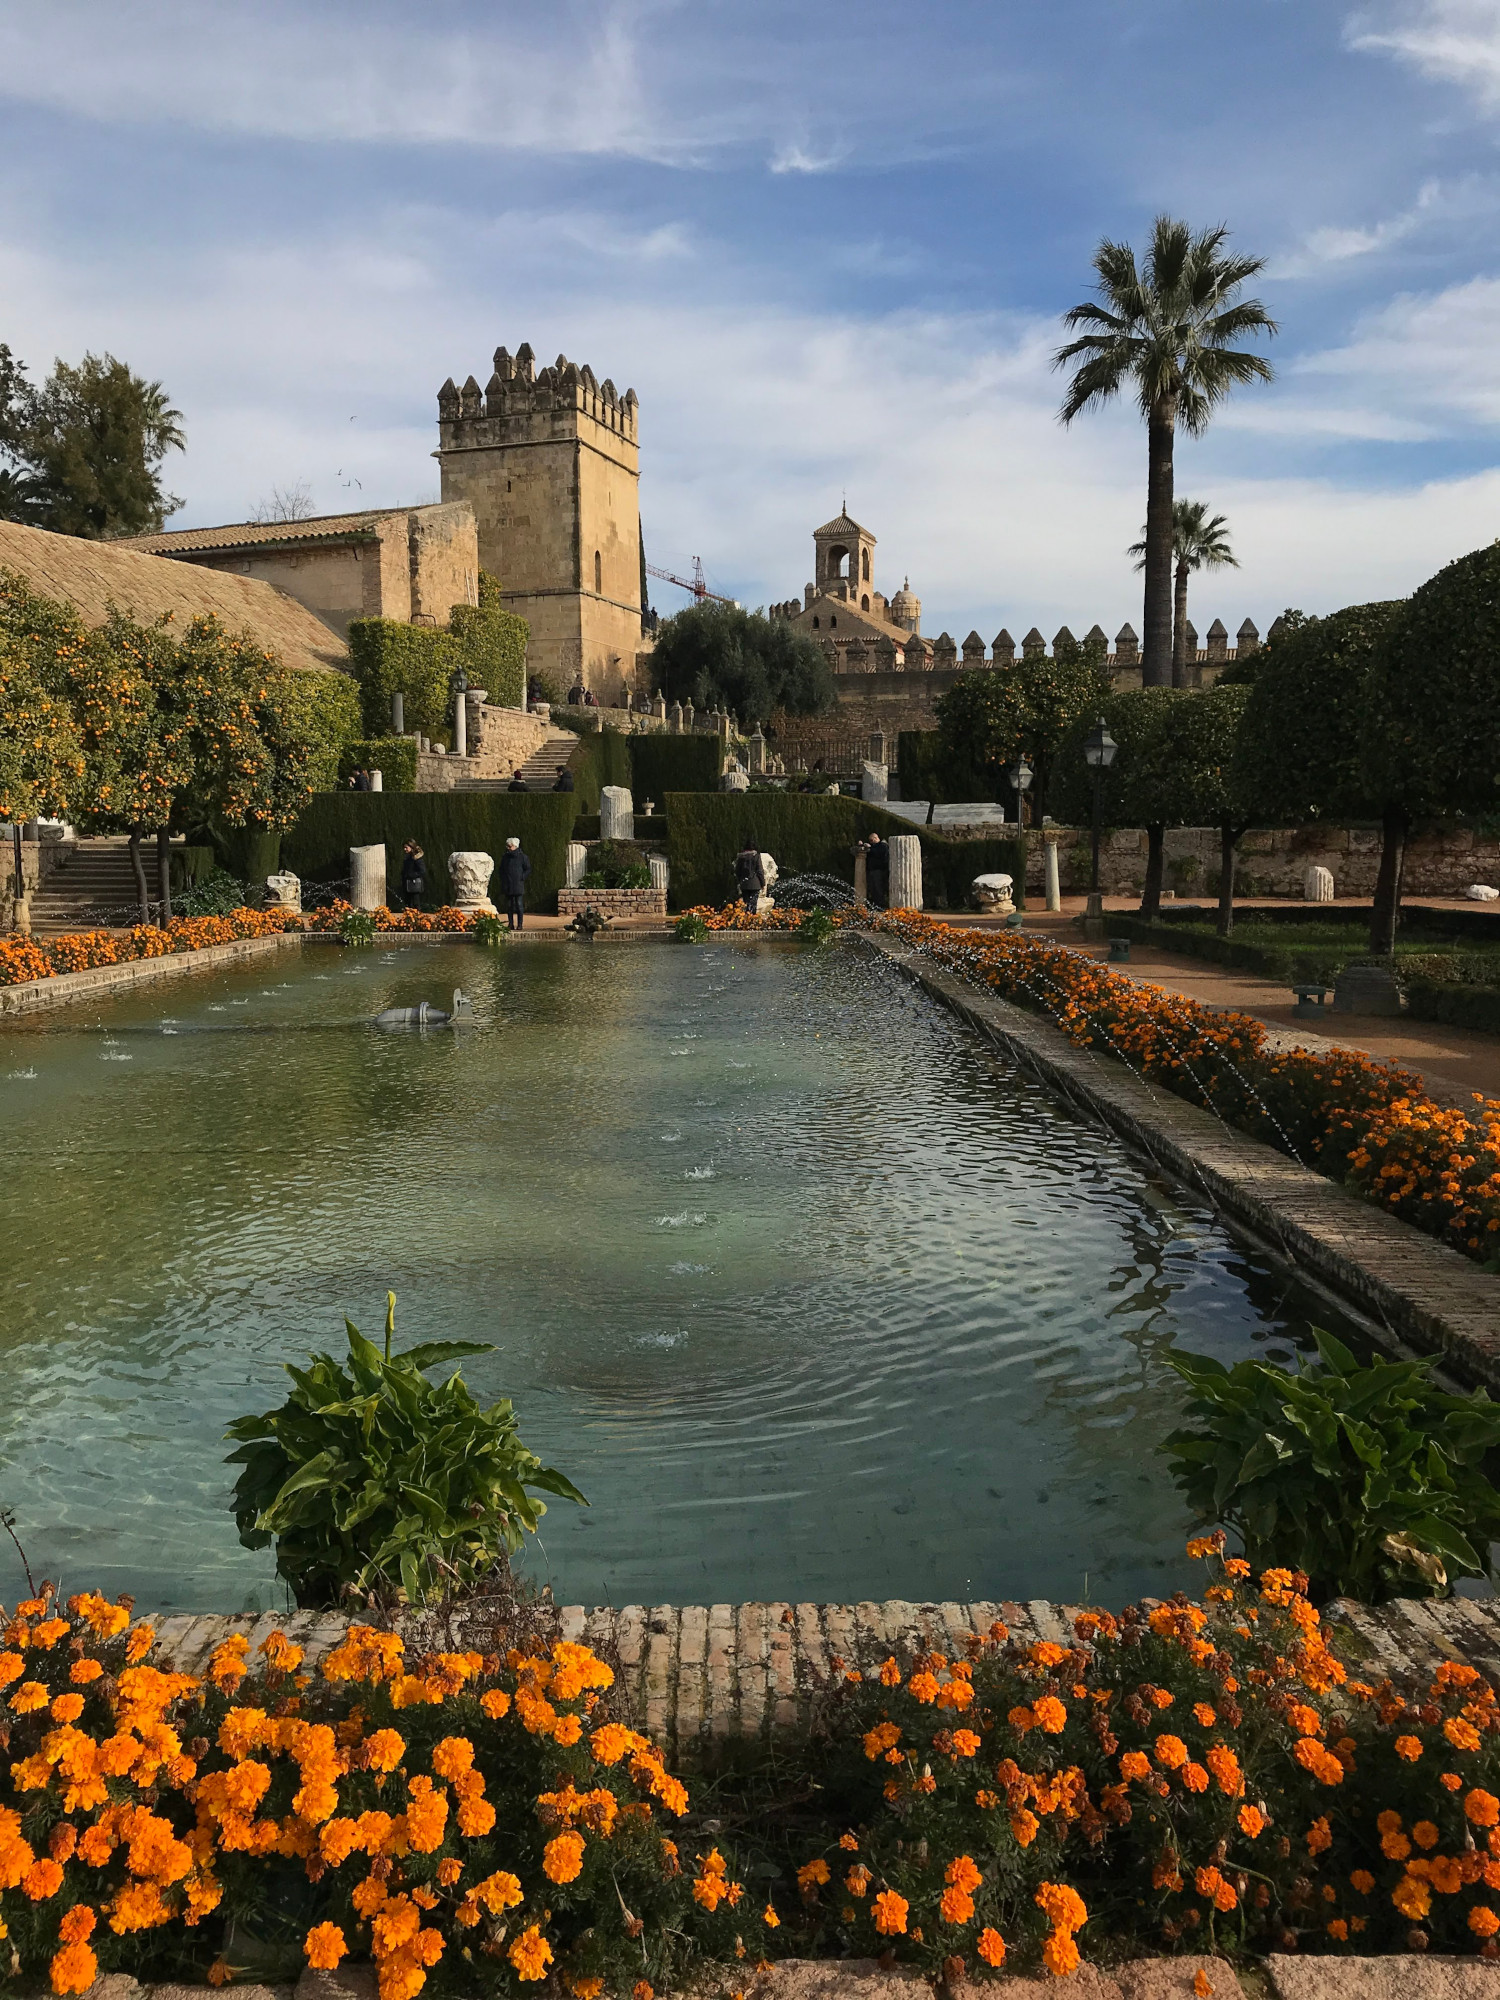
\includegraphics[width=\linewidth]{figures/examples/Alcazar_Cordoba.jpg}
    \caption[Alcázar de los reyes cristianos, Córdoba.]{Alcázar de los reyes cristianos, Córdoba. \href{https://es.wikipedia.org/wiki/Archivo:Alcazar_Cordoba.jpg}{Ahura klik}.}
    \label{fig:apxA:cordoba}
\end{figure}



In vestibulum faucibus ligula eget blandit. Donec eget cursus risus, quis suscipit justo. Curabitur efficitur, dolor nec pulvinar pellentesque, lectus eros hendrerit nisi, in aliquet erat nunc non ipsum. Curabitur felis nunc, viverra nec quam ultrices, suscipit condimentum nibh. Nam faucibus felis hendrerit imperdiet maximus. Curabitur tincidunt porttitor lectus quis feugiat. Sed imperdiet bibendum mi.

\begin{description}
    \item[Nullam quis lacus] vel ante feugiat efficitur id ut quam. Pellentesque commodo elit nec urna gravida maximus. Suspendisse ut risus eu ipsum porta porta ac et orci. Donec dictum ligula sodales, euismod est sed, semper libero \glsname{fiducial}. 
    \item[In blandit], nulla et elementum pharetra, mi nunc sagittis tellus, sit amet scelerisque magna elit ac sapien. Curabitur ipsum dui, pretium a maximus id, varius gravida nisl. Sed vitae mattis elit, vitae hendrerit lorem \cite{IEEE315}.
\end{description}

\subsubsection{Lorem ipsum dolor sit amet, consectetur adipiscing elit}

Integer tempus quis elit id sagittis. Cras tincidunt nisi at tellus luctus, et congue dolor posuere. Aliquam suscipit felis sit amet lacus ultrices aliquet. Sed sagittis ultrices nisi, vel elementum elit dignissim non. 

\subsubsection{Fusce faucibus ex at massa ultrices elementum}

Nullam ullamcorper lorem sit amet facilisis cursus. Suspendisse non erat non justo porta placerat. Morbi porttitor dictum molestie. Sed vitae iaculis libero. Suspendisse in gravida lacus, tempor ultrices nibh. Nam consequat scelerisque porttitor.

\section{Nulla elementum orci in dolor dapibus}

Nulla elementum orci in dolor dapibus, ac facilisis sem ultrices. Nullam eleifend id eros sed luctus. Maecenas arcu ipsum, scelerisque id lorem in, placerat posuere tellus. Etiam gravida velit sed arcu viverra dapibus. Mauris vitae augue dapibus, molestie justo eget, condimentum ipsum. Nulla tristique mi eget semper luctus. Etiam commodo vestibulum vulputate. Etiam quis sapien dolor. Nunc tristique eu lacus quis ullamcorper. Sed volutpat rutrum vehicula. Donec nunc nisl, suscipit in faucibus vitae, tristique eu risus. Nulla facilisis augue eget interdum rutrum. Aliquam sem nunc, fermentum sed urna ac, faucibus interdum nisi.

\subsection{Non luctus mi sollicitudin}

Nam ac tellus ut eros sollicitudin luctus at ac mi. Vestibulum mollis nec nisi a laoreet. Proin neque tortor, placerat nec suscipit sit amet, ullamcorper in sem. Fusce faucibus ultrices cursus. Maecenas scelerisque mauris diam, at volutpat nisi porta vitae. Sed at ipsum et leo cursus varius eu eu lectus. Class aptent taciti sociosqu ad litora torquent per conubia nostra, per inceptos himenaeos. Ut felis ipsum, imperdiet rhoncus orci ac, consectetur luctus nisl. Cras aliquet elementum tellus ullamcorper malesuada. Integer purus est, pharetra eu ullamcorper quis, imperdiet non turpis.

In vestibulum faucibus ligula eget blandit. Donec eget cursus risus, quis suscipit justo. Curabitur efficitur \autoref{code:apx:a:python}, dolor nec pulvinar pellentesque, lectus eros hendrerit nisi, in aliquet erat nunc non ipsum. Curabitur felis nunc, viverra nec quam ultrices, suscipit condimentum nibh. Nam faucibus felis hendrerit imperdiet maximus. Curabitur tincidunt porttitor lectus quis feugiat. Sed imperdiet bibendum mi. Cras aliquet elementum tellus ullamcorper malesuada. Integer purus est, pharetra eu ullamcorper quis, imperdiet non turpis. Sed at ipsum et leo cursus varius eu eu lectus. Class aptent taciti sociosqu ad litora torquent per conubia nostra, per inceptos himenaeos. Curabitur felis nunc, viverra nec quam ultrices, suscipit condimentum nibh. Nam faucibus felis hendrerit imperdiet maximus. Curabitur tincidunt porttitor lectus quis feugiat. 

% [caption={Some Python Code \cite{esp32_devkit_reference_design}}
\begin{code}
\captionof{listing}{Some example large code}
\label{code:apx:a:python}
\begin{minted}{python}
"""
Some interesting python code 
Blah Blah Blah
"""

import numpy as np
from matplotlib import pyplot as plt
from numpy.polynomial import Polynomial as Poly

plt.rcParams["font.family"] = "Libertinus Serif"
plt.rcParams['font.size'] = 14
plt.rcParams['mathtext.fontset'] = 'custom'
plt.rcParams['mathtext.rm'] = 'Libertinus Serif'
plt.rcParams['mathtext.it'] = 'Libertinus Serif:italic'
plt.rcParams['mathtext.bf'] = 'Libertinus Serif:bold'

R510 = 508.3  # Ohms
V5 = 5.018  # Volts

# Open files

nmos_vgs, nmos_vr = np.loadtxt('nmos_ids_vgs.csv', delimiter='\t', unpack=True, skiprows=1)
nmos_sim_vgs, nmos_sim_ids = np.loadtxt('CIC_P0_NMOS_ids_vgs_5.txt', delimiter='\t', unpack=True, skiprows=1)

# Do thingies

nmos_ids = nmos_vr / R510  # Current in resistor
p = Poly.fit(nmos_vgs, nmos_ids, 1)  # Tendency line
print(f"f(x) = {p:unicode}")

# Plot stuff

fig0, ax0 = plt.subplots(figsize=[12, 6])
x = np.linspace(0, 6, 100)

plt.plot(nmos_vgs, nmos_ids, linestyle='none', marker=".", label='Experimental')
plt.plot(nmos_sim_vgs, nmos_sim_ids, linestyle='dashdot', label='Simulation')
plt.plot(x, p(x), linestyle='dashed', label='Tendency')

ax0.grid(True, which='major', color='#DDDDDD', linestyle='-', linewidth=0.6)
ax0.grid(True, which='minor', color='#DDDDDD', linestyle=':', linewidth=0.6)
ax0.minorticks_on()

ax0.legend()

plt.title(r'NMOS, curve $I_{DS}$ / $V_{GS}$')
plt.xlabel(r'$V_{GS}$ (V)')
plt.ylabel(r'$I_{DS}$ (A)')

plt.xlim([0, 6])

# Dont forget to save

plt.savefig("nmos_vgs_ids.pdf")
\end{minted}
\end{code}


    % 
%            ,,                                        
%          `7MM            _.o9                                
%            MM                                             
%  ,6"Yb.    MM  ,p6"bo   ,6"Yb.  M"""MMV  ,6"Yb.  `7Mb,od8 
% 8)   MM    MM 6M'  OO  8)   MM  '  AMV  8)   MM    MM' "' 
%  ,pm9MM    MM 8M        ,pm9MM    AMV    ,pm9MM    MM     
% 8M   MM    MM YM.    , 8M   MM   AMV  , 8M   MM    MM     
% `Moo9^Yo..JMML.YMbmd'  `Moo9^Yo.AMMmmmM `Moo9^Yo..JMML.   
% 
% 
% Free and Open-Source template for academic works
% https://github.com/dpmj/alcazar


% Example of another appendix




\chapter{A long table of things}

Lorem ipsum dolor sit amet, consectetur adipiscing elit. Integer tempus quis elit id sagittis. Cras tincidunt nisi at tellus luctus, et congue dolor posuere. Aliquam suscipit felis sit amet lacus ultrices aliquet. Sed sagittis ultrices nisi, vel elementum elit dignissim non. Fusce faucibus ex at massa ultrices elementum. Nullam ullamcorper lorem sit amet facilisis cursus. Suspendisse non erat non justo porta placerat. Morbi porttitor dictum molestie. Sed vitae iaculis libero. Suspendisse in gravida lacus, tempor ultrices nibh. Nam consequat scelerisque porttitor \footnote{And if you can believe it, It's a Friday once again!}.

Nulla elementum orci in dolor dapibus, ac facilisis sem ultrices. Nullam eleifend id eros sed luctus. Maecenas arcu ipsum, scelerisque id lorem in, placerat posuere tellus. 

Etiam gravida velit sed arcu viverra dapibus. Mauris vitae augue dapibus, molestie justo eget, condimentum ipsum. Nulla tristique mi eget semper luctus \autoref{tab:predecesoras-1}. 


\begin{landscape}
    \begin{table}[p]
    \scriptsize
    \centering
    \renewcommand{\arraystretch}{1.2}
    
    \caption{Example of a long landscape table.}
    \label{tab:predecesoras-1}
    \begin{tabular}{|l|l|p{5.5cm}|l|l|l|l|l|p{5.5cm}|}
    \hline
    \textbf{Nº} & \textbf{EDT} & \textbf{Nombre de tarea} & \textbf{Trabajo} & \textbf{Duración} & \textbf{Predecesoras} & \textbf{Comienzo} & \textbf{Fin} & \textbf{Recursos} \\ \hline\hline
    \textbf{1} & \textbf{1} & \textbf{Dirección del proyecto} & 4 días & 4 días &  & lun 03/07/23 & jue 06/07/23 &  \\ \hline
    2 & 1.1 & Reunión inicial de planificación con el cliente & 3 días & 3 días &  & lun 03/07/23 & mié 05/07/23 & Ana Torres;Carla Aguilar;Diego Ortiz;Lucía   Castro;Martina Martinez;Pablo Gómez;Rodrigo García \\ \hline
    3 & 1.2 & Reparto de tareas a los trabajadores & 1 día & 1 día & 1.1 & jue 06/07/23 & jue 06/07/23 & Ana Torres \\ \hline
    \textbf{4} & \textbf{2} & \textbf{Estudio de la viabilidad del despliegue} & \textbf{27 días} & \textbf{9,67 días} & \textbf{} & \textbf{vie 07/07/23} & \textbf{jue 20/07/23} & \textbf{} \\ \hline
    5 & 2.1 & Estudio de la orografía & 5 días & 1,67 días & 1.2 & vie 07/07/23 & lun 10/07/23 & Rodrigo García;Paloma Cuesta;Ramón García \\ \hline
    6 & 2.2 & Estudio del emplazamiento de las antenas del   radioenlace y balance de potencias & 4 días & 1,33 días & 2.1 & mié 12/07/23 & jue 13/07/23 & Rodrigo García;Paloma Cuesta;Ramón García \\ \hline
    7 & 2.3 & Estudio del emplazamiento de las estaciones   base y radio de cobertura & 4 días & 1,33 días & 2.1 & jue 13/07/23 & vie 14/07/23 & Rodrigo García;Paloma Cuesta;Ramón García \\ \hline
    8 & 2.4 & Estudio de la magnitud del tráfico & 3 días & 1 día & 1.2 & lun 10/07/23 & mar 11/07/23 & Rodrigo García;Paloma Cuesta;Ramón García \\ \hline
    9 & 2.5 & Revisión de la normativa & 2 días & 0,67 días & 1.2 & mar 11/07/23 & mié 12/07/23 & Rodrigo García;Paloma Cuesta;Ramón García \\ \hline
    10 & 2.6 & Establecimiento de los requisitos técnicos & 5 días & 1,67 días & 2.1;2.2;2.3;2.4;2.5 & lun 17/07/23 & mar 18/07/23 & Rodrigo García;Paloma Cuesta;Ramón García \\ \hline
    11 & 2.7 & Establecimiento de un presupuesto temprano & 4 días & 2 días & 2.6 & mar 18/07/23 & jue 20/07/23 & Ana Torres;Rodrigo García \\ \hline
    \textbf{12} & \textbf{3} & \textbf{Diseño del despliegue} & \textbf{41 días} & \textbf{14 días} & \textbf{} & \textbf{jue 20/07/23} & \textbf{mié 09/08/23} & \textbf{} \\ \hline
    13 & 3.1 & Diseño de la red & 29 días & 9,67 días &  & jue 20/07/23 & jue 03/08/23 &  \\ \hline
    14 & 3.1.1 & Diseño de las estaciones base de telefonía & 7 días & 9,67 días &  & jue 20/07/23 & jue 03/08/23 &  \\ \hline
    15 & 3.1.1.1 & Elección del emplazamiento físico & 5 días & 1,67 días & 2 & jue 20/07/23 & lun 24/07/23 & Rodrigo García;Paloma Cuesta;Ramón García \\ \hline
    16 & 3.1.1.2 & Diseño de la sectorización y el apuntado & 2 días & 0,67 días & 3.1.1.1 & mié 02/08/23 & jue 03/08/23 & Rodrigo García;Paloma Cuesta;Ramón García \\ \hline
    17 & 3.1.2 & Diseño de las estaciones base del radioenlace & 7 días & 2,33 días &  & lun 24/07/23 & mié 26/07/23 &  \\ \hline
    18 & 3.1.2.1 & Elección del emplazamiento físico & 5 días & 1,67 días & 2 & lun 24/07/23 & mar 25/07/23 & Rodrigo García;Paloma Cuesta;Ramón García \\ \hline
    19 & 3.1.2.2 & Diseño del apuntado & 2 días & 0,67 días & 3.1.2.1 & mié 26/07/23 & mié 26/07/23 & Rodrigo García;Paloma Cuesta;Ramón García \\ \hline
    20 & 3.1.3 & Diseño de la topología de red & 10 días & 3,33 días & 2 & mié 26/07/23 & lun 31/07/23 & Rodrigo García;Paloma Cuesta;Ramón García \\ \hline
    21 & 3.1.4 & Diseño de la gestión y separación del tráfico & 5 días & 1,67 días & 2 & mar 01/08/23 & mié 02/08/23 & Rodrigo García;Paloma Cuesta;Ramón García \\ \hline
    22 & 3.2 & Elección de equipos y componentes & 10 días & 3,33 días &  & jue 03/08/23 & mar 08/08/23 &  \\ \hline
    23 & 3.2.1 & Elección de los equipos de RF & 5 días & 1,67 días & 3.1 & jue 03/08/23 & vie 04/08/23 & Rodrigo García;Paloma Cuesta;Ramón García \\ \hline
    24 & 3.2.2 & Elección de los equipos de red & 5 días & 1,67 días & 3.1 & lun 07/08/23 & mar 08/08/23 & Rodrigo García;Paloma Cuesta;Ramón García \\ \hline
    25 & 3.3 & Elaboración del presupuesto base & 2 días & 1 día & 3.1;3.2 & mar 08/08/23 & mié 09/08/23 & Rodrigo García;Ana Torres \\ \hline
    \textbf{26} & \textbf{4} & \textbf{Despliegue físico} & \textbf{38 días} & \textbf{15,83 días} & \textbf{} & \textbf{mié 09/08/23} & \textbf{jue 31/08/23} & \textbf{} \\ \hline
    27 & 4.1 & Reunión de materiales & 4 días & 2 días & 3 & mié 09/08/23 & vie 11/08/23 & Diego Ortiz;Martina Martinez \\ \hline
    28 & 4.2 & Construcción & 15 días & 7,5 días &  & vie 11/08/23 & mié 23/08/23 &  \\ \hline
    29 & 4.2.1 & Estaciones de telefonía & 5 días & 2,5 días & 4.1 & vie 11/08/23 & mié 16/08/23 & Diego Ortiz;Martina Martinez \\ \hline
    \end{tabular}%
    \end{table}
\end{landscape}
    % 
%            ,,                                        
%          `7MM            _.o9                                
%            MM                                             
%  ,6"Yb.    MM  ,p6"bo   ,6"Yb.  M"""MMV  ,6"Yb.  `7Mb,od8 
% 8)   MM    MM 6M'  OO  8)   MM  '  AMV  8)   MM    MM' "' 
%  ,pm9MM    MM 8M        ,pm9MM    AMV    ,pm9MM    MM     
% 8M   MM    MM YM.    , 8M   MM   AMV  , 8M   MM    MM     
% `Moo9^Yo..JMML.YMbmd'  `Moo9^Yo.AMMmmmM `Moo9^Yo..JMML.   
% 
% 
% Free and Open-Source template for academic works
% https://github.com/dpmj/alcazar



% ------------------------------------------------------------------------------
% SUSTAINABLE DEVELOPMENT GOALS
% An example of usage, in case your university requires them.


\chapter{Sustainable Development Goals}

The Sustainable Development Goals are a collection of seventeen interlinked objectives designed to serve as a ``\textit{shared blueprint for peace and prosperity for people and the planet, now and into the future}''. This project is in line with the following Sustainable Development Goals:



% Remove the SDGs that you see fit

\begin{multicols}{2}
    
    \small
    \setlength\tabcolsep{0pt}
    \renewcommand*{\arraystretch}{1}

    \noindent
    \begin{tabular}{p{25mm} p{46mm}}
        \vspace{0mm} 
\includegraphics[width=2cm]{text/appendix/appendix-sdg/resources/sdg1.pdf} & \vspace{-0.5mm} \textbf{1. No poverty.} End poverty in all its forms everywhere. In vestibulum faucibus ligula eget blandit. Donec eget cursus risus, quis suscipit justo. \\
    \end{tabular}

    \noindent
    \begin{tabular}{p{25mm} p{46mm}}
        \vspace{0mm} 
\includegraphics[width=2cm]{text/appendix/appendix-sdg/resources/sdg2.pdf} & \vspace{-0.5mm} \textbf{2. Zero hunger.} End hunger, achieve food security and improved nutrition and promote sustainable agriculture. Nulla elementum orci in dolor. \\
    \end{tabular}

    \noindent
    \begin{tabular}{p{25mm} p{46mm}}
        \vspace{0mm} 
\includegraphics[width=2cm]{text/appendix/appendix-sdg/resources/sdg3.pdf} & \vspace{-0.5mm} \textbf{3. Good health and well-being.} Ensure healthy lives and promote well-being for all at all ages. Molestie justo eget, condimentum ipsum.\\
    \end{tabular}

    \noindent
    \begin{tabular}{p{25mm} p{46mm}}
        \vspace{0mm} 
\includegraphics[width=2cm]{text/appendix/appendix-sdg/resources/sdg4.pdf} & \vspace{-0.5mm} \textbf{4. Quality education.} Ensure inclusive and equitable quality education and promote lifelong learning opportunities for all. \\
    \end{tabular}

    \noindent
    \begin{tabular}{p{25mm} p{46mm}}
        \vspace{0mm} 
\includegraphics[width=2cm]{text/appendix/appendix-sdg/resources/sdg5.pdf} & \vspace{-0.5mm} \textbf{5. Gender equality.} Achieve gender equality and empower all women and girls.  \\
    \end{tabular}

    \noindent
    \begin{tabular}{p{25mm} p{46mm}}
        \vspace{0mm} 
\includegraphics[width=2cm]{text/appendix/appendix-sdg/resources/sdg6.pdf} & \vspace{-0.5mm} \textbf{6. Clean water and sanitation.} Ensure availability and sustainable management of water and sanitation for all.\\
    \end{tabular}

    \noindent
    \begin{tabular}{p{25mm} p{46mm}}
        \vspace{0mm} 
\includegraphics[width=2cm]{text/appendix/appendix-sdg/resources/sdg7.pdf} & \vspace{-0.5mm} \textbf{7. Affordable and clean energy.} Ensure access to affordable, reliable, sustainable and modern energy for all. Donec dictum ligula sodales, euismod est sed, semper libero.  \\
    \end{tabular}

    \noindent
    \begin{tabular}{p{25mm} p{46mm}}
        \vspace{0mm} 
\includegraphics[width=2cm]{text/appendix/appendix-sdg/resources/sdg8.pdf} & \vspace{-0.5mm} \textbf{8. Decent work and economic growth.} Promote sustained, inclusive and sustainable economic growth, full and productive employment and decent work for all. \\
    \end{tabular}

    \noindent
    \begin{tabular}{p{25mm} p{46mm}}
        \vspace{0mm} 
\includegraphics[width=2cm]{text/appendix/appendix-sdg/resources/sdg9.pdf} & \vspace{-0.5mm} \textbf{9. Industry, Innovation and Infrastructure.} Build resilient infrastructure, promote inclusive and sustainable industrialization and foster innovation. \\
    \end{tabular}

    \noindent
    \begin{tabular}{p{25mm} p{46mm}}
        \vspace{0mm} 
\includegraphics[width=2cm]{text/appendix/appendix-sdg/resources/sdg10.pdf} & \vspace{-0.5mm} \textbf{10. Reduced inequality.} Reduce inequality within and among countries. Donec eget cursus risus, quis suscipit justo. \\
    \end{tabular}

    \noindent
    \begin{tabular}{p{25mm} p{46mm}}
        \vspace{0mm} 
\includegraphics[width=2cm]{text/appendix/appendix-sdg/resources/sdg11.pdf} & \vspace{-0.5mm} \textbf{11. Sustainable cities and communities.} Make cities and human settlements inclusive, safe, resilient and sustainable. \\
    \end{tabular}

    \noindent
    \begin{tabular}{p{25mm} p{46mm}}
        \vspace{0mm} 
\includegraphics[width=2cm]{text/appendix/appendix-sdg/resources/sdg12.pdf} & \vspace{-0.5mm} \textbf{12. Responsible consumption and production.} Ensure sustainable consumption and production patterns. \\
    \end{tabular}

    \noindent
    \begin{tabular}{p{25mm} p{46mm}}
        \vspace{0mm} 
\includegraphics[width=2cm]{text/appendix/appendix-sdg/resources/sdg13.pdf} & \vspace{-0.5mm} \textbf{13. Climate action.} Take urgent action to combat climate change and its impacts.  \\
    \end{tabular}

    \noindent
    \begin{tabular}{p{25mm} p{46mm}}
        \vspace{0mm} 
\includegraphics[width=2cm]{text/appendix/appendix-sdg/resources/sdg14.pdf} & \vspace{-0.5mm} \textbf{14. Life below water.} Conserve and sustainably use the oceans, seas and marine resources for sustainable development. \\
    \end{tabular}

\end{multicols}


    \newpage


\begin{multicols}{2}

    \small
    \setlength\tabcolsep{0pt}
    \renewcommand*{\arraystretch}{1}

    \noindent
    \begin{tabular}{p{25mm} p{46mm}}
        \vspace{0mm} 
\includegraphics[width=2cm]{text/appendix/appendix-sdg/resources/sdg15.pdf} & \vspace{-0.5mm} \textbf{15. Life on land.} Protect, restore and promote sustainable use of terrestrial ecosystems, sustainably manage forests, combat desertification, and halt and reverse land degradation and halt biodiversity loss. \\
    \end{tabular}

    \noindent
    \begin{tabular}{p{25mm} p{46mm}}
        \vspace{0mm} 
\includegraphics[width=2cm]{text/appendix/appendix-sdg/resources/sdg16.pdf} & \vspace{-0.5mm} \textbf{16. Peace, justice and strong institutions.} Promote peaceful and inclusive societies for sustainable development, provide access to justice for all and build effective, accountable and inclusive institutions at all levels. \\
    \end{tabular}

    \noindent
    \begin{tabular}{p{25mm} p{46mm}}
        \vspace{0mm} 
\includegraphics[width=2cm]{text/appendix/appendix-sdg/resources/sdg17.pdf} & \vspace{-0.5mm} \textbf{17. Partnership for the goals.} Strengthen the means of implementation and revitalize the Global Partnership for Sustainable Development. \\
    \end{tabular}

\end{multicols}  % Sustainable Development Goals Appendix

\end{appendices}




% It's nice to say thanks. 
%% 
%            ,,                                        
%          `7MM            _.o9                                
%            MM                                             
%  ,6"Yb.    MM  ,p6"bo   ,6"Yb.  M"""MMV  ,6"Yb.  `7Mb,od8 
% 8)   MM    MM 6M'  OO  8)   MM  '  AMV  8)   MM    MM' "' 
%  ,pm9MM    MM 8M        ,pm9MM    AMV    ,pm9MM    MM     
% 8M   MM    MM YM.    , 8M   MM   AMV  , 8M   MM    MM     
% `Moo9^Yo..JMML.YMbmd'  `Moo9^Yo.AMMmmmM `Moo9^Yo..JMML.   
% 
% 
% Free and Open-Source template for academic works
% https://github.com/dpmj/alcazar


% It's nice to say thanks


\newpage
\clearpage
\cleardoublepage

\thispagestyle{empty}

\vspace*{\fill}

\begin{center}
    \textbf{\large Thank you for reading this {\thesisType}.}
    \vspace{1cm}
\end{center}

\vspace*{\fill}


  % Comment this line if you feel like it.

\end{document}

% END DOCUMENT
% %%%%%%%%%%%%%%%%%%%%%%%%%%%%%%%%%%%%%%%%%%%%%%%%%%%%%%%%%%%%%%%%%%%%%%%%%%%%%%


